% Options for packages loaded elsewhere
\PassOptionsToPackage{unicode}{hyperref}
\PassOptionsToPackage{hyphens}{url}
\PassOptionsToPackage{dvipsnames,svgnames,x11names}{xcolor}
%
\documentclass[
  singlecolumn]{report}

\usepackage{amsmath,amssymb}
\usepackage{iftex}
\ifPDFTeX
  \usepackage[T1]{fontenc}
  \usepackage[utf8]{inputenc}
  \usepackage{textcomp} % provide euro and other symbols
\else % if luatex or xetex
  \usepackage{unicode-math}
  \defaultfontfeatures{Scale=MatchLowercase}
  \defaultfontfeatures[\rmfamily]{Ligatures=TeX,Scale=1}
\fi
\usepackage[]{libertinus}
\ifPDFTeX\else  
    % xetex/luatex font selection
\fi
% Use upquote if available, for straight quotes in verbatim environments
\IfFileExists{upquote.sty}{\usepackage{upquote}}{}
\IfFileExists{microtype.sty}{% use microtype if available
  \usepackage[]{microtype}
  \UseMicrotypeSet[protrusion]{basicmath} % disable protrusion for tt fonts
}{}
\makeatletter
\@ifundefined{KOMAClassName}{% if non-KOMA class
  \IfFileExists{parskip.sty}{%
    \usepackage{parskip}
  }{% else
    \setlength{\parindent}{0pt}
    \setlength{\parskip}{6pt plus 2pt minus 1pt}}
}{% if KOMA class
  \KOMAoptions{parskip=half}}
\makeatother
\usepackage{xcolor}
\usepackage[top=30mm,left=20mm,heightrounded]{geometry}
\setlength{\emergencystretch}{3em} % prevent overfull lines
\setcounter{secnumdepth}{-\maxdimen} % remove section numbering
% Make \paragraph and \subparagraph free-standing
\ifx\paragraph\undefined\else
  \let\oldparagraph\paragraph
  \renewcommand{\paragraph}[1]{\oldparagraph{#1}\mbox{}}
\fi
\ifx\subparagraph\undefined\else
  \let\oldsubparagraph\subparagraph
  \renewcommand{\subparagraph}[1]{\oldsubparagraph{#1}\mbox{}}
\fi


\providecommand{\tightlist}{%
  \setlength{\itemsep}{0pt}\setlength{\parskip}{0pt}}\usepackage{longtable,booktabs,array}
\usepackage{calc} % for calculating minipage widths
% Correct order of tables after \paragraph or \subparagraph
\usepackage{etoolbox}
\makeatletter
\patchcmd\longtable{\par}{\if@noskipsec\mbox{}\fi\par}{}{}
\makeatother
% Allow footnotes in longtable head/foot
\IfFileExists{footnotehyper.sty}{\usepackage{footnotehyper}}{\usepackage{footnote}}
\makesavenoteenv{longtable}
\usepackage{graphicx}
\makeatletter
\def\maxwidth{\ifdim\Gin@nat@width>\linewidth\linewidth\else\Gin@nat@width\fi}
\def\maxheight{\ifdim\Gin@nat@height>\textheight\textheight\else\Gin@nat@height\fi}
\makeatother
% Scale images if necessary, so that they will not overflow the page
% margins by default, and it is still possible to overwrite the defaults
% using explicit options in \includegraphics[width, height, ...]{}
\setkeys{Gin}{width=\maxwidth,height=\maxheight,keepaspectratio}
% Set default figure placement to htbp
\makeatletter
\def\fps@figure{htbp}
\makeatother
\newlength{\cslhangindent}
\setlength{\cslhangindent}{1.5em}
\newlength{\csllabelwidth}
\setlength{\csllabelwidth}{3em}
\newlength{\cslentryspacingunit} % times entry-spacing
\setlength{\cslentryspacingunit}{\parskip}
\newenvironment{CSLReferences}[2] % #1 hanging-ident, #2 entry spacing
 {% don't indent paragraphs
  \setlength{\parindent}{0pt}
  % turn on hanging indent if param 1 is 1
  \ifodd #1
  \let\oldpar\par
  \def\par{\hangindent=\cslhangindent\oldpar}
  \fi
  % set entry spacing
  \setlength{\parskip}{#2\cslentryspacingunit}
 }%
 {}
\usepackage{calc}
\newcommand{\CSLBlock}[1]{#1\hfill\break}
\newcommand{\CSLLeftMargin}[1]{\parbox[t]{\csllabelwidth}{#1}}
\newcommand{\CSLRightInline}[1]{\parbox[t]{\linewidth - \csllabelwidth}{#1}\break}
\newcommand{\CSLIndent}[1]{\hspace{\cslhangindent}#1}

\usepackage{cancel}
\makeatletter
\makeatother
\makeatletter
\makeatother
\makeatletter
\@ifpackageloaded{caption}{}{\usepackage{caption}}
\AtBeginDocument{%
\ifdefined\contentsname
  \renewcommand*\contentsname{Table of contents}
\else
  \newcommand\contentsname{Table of contents}
\fi
\ifdefined\listfigurename
  \renewcommand*\listfigurename{List of Figures}
\else
  \newcommand\listfigurename{List of Figures}
\fi
\ifdefined\listtablename
  \renewcommand*\listtablename{List of Tables}
\else
  \newcommand\listtablename{List of Tables}
\fi
\ifdefined\figurename
  \renewcommand*\figurename{Figure}
\else
  \newcommand\figurename{Figure}
\fi
\ifdefined\tablename
  \renewcommand*\tablename{Table}
\else
  \newcommand\tablename{Table}
\fi
}
\@ifpackageloaded{float}{}{\usepackage{float}}
\floatstyle{ruled}
\@ifundefined{c@chapter}{\newfloat{codelisting}{h}{lop}}{\newfloat{codelisting}{h}{lop}[chapter]}
\floatname{codelisting}{Listing}
\newcommand*\listoflistings{\listof{codelisting}{List of Listings}}
\makeatother
\makeatletter
\@ifpackageloaded{caption}{}{\usepackage{caption}}
\@ifpackageloaded{subcaption}{}{\usepackage{subcaption}}
\makeatother
\makeatletter
\@ifpackageloaded{tcolorbox}{}{\usepackage[skins,breakable]{tcolorbox}}
\makeatother
\makeatletter
\@ifundefined{shadecolor}{\definecolor{shadecolor}{rgb}{.97, .97, .97}}
\makeatother
\makeatletter
\makeatother
\makeatletter
\makeatother
\ifLuaTeX
  \usepackage{selnolig}  % disable illegal ligatures
\fi
\IfFileExists{bookmark.sty}{\usepackage{bookmark}}{\usepackage{hyperref}}
\IfFileExists{xurl.sty}{\usepackage{xurl}}{} % add URL line breaks if available
\urlstyle{same} % disable monospaced font for URLs
\hypersetup{
  pdftitle={How to Construct Causal Diagrams (DAGS) in Cultural Evolutionary Research},
  pdfauthor={Joseph A. Bulbulia},
  colorlinks=true,
  linkcolor={blue},
  filecolor={Maroon},
  citecolor={Blue},
  urlcolor={Blue},
  pdfcreator={LaTeX via pandoc}}

\title{How to Construct Causal Diagrams (DAGS) in Cultural Evolutionary
Research}
\author{Joseph A. Bulbulia}
\date{}

\begin{document}
\maketitle
\ifdefined\Shaded\renewenvironment{Shaded}{\begin{tcolorbox}[enhanced, sharp corners, breakable, borderline west={3pt}{0pt}{shadecolor}, interior hidden, boxrule=0pt, frame hidden]}{\end{tcolorbox}}\fi

\listoffigures
\listoftables
\hypertarget{abstract}{%
\section{Abstract}\label{abstract}}

\hypertarget{introduction}{%
\section{Introduction}\label{introduction}}

Correlation is not causation. However, across many human sciences,
persistent confusion in the analysis and reporting of correlations has
limited scientific progress. The direction of causation frequently runs
in the opposite direction to the direction of manifest correlations.
This problem is widely known. Nevertheless, many human scientists report
manifest correlations using hedging language. Making matters worse,
widely adopted strategies for confounding control fail
(\protect\hyperlink{ref-mcelreath2020}{McElreath 2020}), suggesting a
``causality crisis'' (\protect\hyperlink{ref-bulbulia2022}{Bulbulia
2022}). Addressing the causality crisis is arguably among the human
science's most pressing tasks.

When integrated into methodologically rigorous workflows, causal
directed acyclic graphs (``DAGs'', or ``causal diagramms'') can be
powerful tools for clarifying causality.\footnote{The term ``DAG'' is
  unfortunate because not all directed acyclic graphs are causal. For a
  graph to be causal it must satisfy the conditions of markov
  factorisation (see Appendix A).} A system of formal mathematical
proofs underpins their design. This brings confidence. No formal
mathematical training is required to use them. This makes them
accessible. However, causal inference relies on assumptions. causal
diagrams are methods for encoding such assumptions. When assumptions are
unwarrented, causal diagrams may decieve. For example, when researchers
lack time-series data unbiased causal effect estimates are generally not
warrented (\protect\hyperlink{ref-vanderweele2015}{T. VanderWeele
2015a}). Cross-sectional researchers who use causal diagrams to report
their unrealistic assumptions use DAGS as props for unwarrented cover.
Ideally causal diagrams would be equipped with safety mechanisms that
prevent such misapplications.

Here, I present a set of strategies for writing causal diagrams (or
causal diagrams as I will call them) that reduces the scope for
unwarrented use. I call these \emph{chronologically causal graph}, and
offer a tutorial for cultural evolutionary researchers on their use.

There are many excellent introductions to causal diagrams
(\protect\hyperlink{ref-rohrer2018}{Rohrer 2018};
\protect\hyperlink{ref-hernan2023}{Hernan and Robins 2023a};
\protect\hyperlink{ref-cinelli2022}{Cinelli, Forney, and Pearl 2022};
\protect\hyperlink{ref-barrett2021}{Barrett 2021};
\protect\hyperlink{ref-mcelreath2020}{McElreath 2020};
\protect\hyperlink{ref-greenland1999}{Greenland, Pearl, and Robins
1999}; \protect\hyperlink{ref-suzuki2020}{Suzuki, Shinozaki, and
Yamamoto 2020}; \protect\hyperlink{ref-pearl2009}{Pearl
2009}).\footnote{One of the best resources is Miguel Hernan's free
  course, here:
  \url{https://pll.harvard.edu/course/causal-diagrams-draw-your-assumptions-your-conclusions}.}.
One may reasonably ask whether another introduction adds clutter. The
approach I present here adds value in five ways.

In \textbf{Part 1.} , I explain how to effectively leverage causal
diagrams within the framework of counterfactual or ``potential''
outcomes, an approach crucial for conceptualizing causality. In my view,
a significant impediment to causal inference is the common misconception
that it is purely an aspect of manifest data science. Instead, it should
be considered an aspect of what migth be called counterfactual data
science, an approach that formulates and answers quantitative
comparative questions about how the world could have been different from
its current state. Without the ability to ask and resolve such
counterfactual questions, we cannot quantitatively evaluate causal
claims. I devote attention to clarifying the counterfactual
underpinnings of quantitative causal inference because one should not
use causal diagrams without understanding that basis.

In \textbf{Part 2}, I review the four elemental forms of confounding.
Here I show how chronological causal diagrams elucidate strategies for
confounding control. A brief introduction examines

Although this discussion replicates material from other tutorials, by
emphasising the benefits of temporal order in spatial organisation of a
causal graph the conditions in which we may (or may not) identify
causality in the presence of confounding become more apparent. Here, I
briefly show how causal diagrams may clarify poorly understood concepts
of interaction, mediation, and repeated measures longitudinal data.
Chronologically consciencious causal diagrams help us to understand why
commonplace modelling approaches such as multilevel modelling and
structural equation modelling are often poorly suited to the demands of
counterfactual data-science.

In \textbf{Part 3}, I explain how chronological causal diagrams clarify
mission-critical demands for data-collection in three-wave panel
designs.

In \textbf{Part 4}, I focus on the problem of selection bias as it
arises in a three-wave panel, using chronological causal diagrams to
focus attention on the imperatives for (a) adequate sampling and (b)
longitudinal retention.

In \textbf{Part 5}, I focus on the problem of measurement error as it
arises in a three-wave panel, again using chronological causal diagrams
to focus attention on the imperatives for (a) ensuring reliable
measures, (b) assessing pathways for confounding from correlated and
directed measurement errors.

Additional technical details are presented in Appendices.

\hypertarget{part-1.-the-three-fundamental-identifiability-assumption-for-counterfactual-data-science}{%
\section{Part 1. The three fundamental identifiability assumption for
counterfactual data
science}\label{part-1.-the-three-fundamental-identifiability-assumption-for-counterfactual-data-science}}

causal diagrams are powerful tools for answering causal questions.
However before we can answer a causal question we must first understand
how to ask one. In this section I review key concepts and identification
assumptions.

\hypertarget{the-fundamental-problem-of-causal-inference}{%
\subsection{The fundamental problem of causal
inference}\label{the-fundamental-problem-of-causal-inference}}

We say that \(A\) causes \(Y\) if changing \(A\) would have made a
difference to the outcome of \(Y\). The use of the subjective ``would
have'' reveals the need for counterfactual reasoning to conceive of
causal effects. To infer a causality requires a contrast between how the
world as it is and how the world might have been. ``Causal inference''
we aim to quantify the magnitude of differences between the world as it
is, and the world as it might have been.

Suppose there are manifest correlations in the data between cultural
beliefs in Big Gods and social complexity. Suppose further that we are
interested in estimating the causal effect of belief in Big Gods on
social complexity. We call beliefs in Big Gods the ``exposure'' or
``treatment.'' We denote the exposure using the symbol \(A\). We call
social complexity the outcome, denoted by the symbol \(Y\). For now, we
assume the exposure, outcome, and the units (cultures) are well-defined.
Later we shall relax these assumptions.

To assess causality we must define two counterfactual (or ``potential'')
outcomes for each culture in a population of cultures:

\begin{itemize}
\tightlist
\item
  \(Y_i(a = 1)\): The social complexity of culture \(i\) if they
  believed in Big Gods. This is the outcome when \(A_i = 1\). This
  outcoome is counterfactual for culture\(_i\), when the exposure
  \(A_i = 0\).
\item
  \(Y_i(a = 0)\): The social complexity of culture \(i\) if they did not
  believe in Big Gods. This is the counterfactual outcome when
  \(A_i = 0\). This outcoome is counterfactual for culture\(_i\) when
  the exposure \(A_i = 1\).
\end{itemize}

The causal effect of a belief in Big Gods on social complexity for
culture\(_i\) may be defined as a contrast on the difference scale
between two potential outcomes (\(Y_i(a)\)) under the two different
levels of the exposure (\(A_i = 1\) (belief in Big Gods); \(A_i = 0\)
(no belief in Big Gods)). For simplicity we assume these exposures are
exhaustive. Under these assumptions:

\[
\text{Causal Effect of Belief in Big Gods}_i = Y_i(1) - Y_i(0) 
\]

Notice that to assess causality we require a contrast between two states
of the world only one of which any culture might actually realise
\footnote{The counterfactual outcome under the exposure \(A = a\) may be
  written in different ways, such as \(Y(a)\) (the notation we use
  here), \(Y^{a}\), and \(Y_a\).} That is, when a culture receives one
level of a belief in Big Gods the outcome under the other level(s) is
ruled out. That the manifest data present only partial evidence for
quantifying causal contrasts is called ``the fundamental problem of
causal inference''(\protect\hyperlink{ref-rubin1976}{Rubin 1976};
\protect\hyperlink{ref-holland1986}{Holland 1986}). Inferring
counterfactual contrasts is a special case of a \emph{a missing data
problem} (\protect\hyperlink{ref-westreich2015}{Westreich et al. 2015};
\protect\hyperlink{ref-edwards2015}{Edwards, Cole, and Westreich 2015}).

\hypertarget{simulating-average-causal-effects-under-different-exposures-and-contrasting-them-requires-a-counterfactual-data-science.}{%
\subsubsection{Simulating average causal effects under different
exposures and contrasting them requires a counterfactual
data-science.}\label{simulating-average-causal-effects-under-different-exposures-and-contrasting-them-requires-a-counterfactual-data-science.}}

Although we cannot generally observe unit-level causal effects, it may
be possible to estimate average causal effects. We do this by
contrasting the average effect in the population \emph{were all units in
exposed group} with the average effect in the unexposed group \emph{were
all units unexposed} group. Suppose we are interested in estimating this
contrast on the difference scale. We may write this as the difference of
the (1) average outcome were everyone exposed to one level of the
intervention and (2) average outcome were everyone exposed to one level
of the intervention, or equivalently as the average of the
differences.\footnote{Note that mathematically, the difference in the
  average expectation is equivalent to the average of the differences in
  expectation.}

\begin{alignat*}{2}
ATE & = E[(a)) - E(Y(0)]\\
& = E[Y(1) - Y(0)]
\end{alignat*}

The average treatment effects that we are interested in estimating need
not be the effects of binary exposures. We may obtain contrasts between
two different levels of a multinomial or continuous exposure. If we
define the levels we wish to contrast as \(A = a\) and \(A = a*\). Then
the average treatment effect is given by the expression:

   \begin{align*}
    ATE = E[Y(a) - Y(a*)]
    \end{align*}

Recall that generally any unit-level causal effect is not identified in
the data -- we only observe each unit under one or another exposure
level. However, if the following three fundamental identification
assumptions are credible, we may -- by assumption -- obtain these
average (or ``marginal'' contrasts).

The three fundamental identification conditions for causal inference,
when they obtain, allow researchers to recover the counterfactual
contrasts necessary to compute causal effects from observed data. Not
only does causal estimation rely on assumptions about the causal
relationships that researchers hope to estimate, the data are generally
insufficient to fully assess the fundamental identifibility assumptions
on which causal estimation relies. Note that these assumptions are
implicit in randomised experimental designs.

\hypertarget{identification-assumption-1-causal-consistency}{%
\subsubsection{Identification assumption 1: causal
consistency}\label{identification-assumption-1-causal-consistency}}

We satisfy the causal consistency assumption when the potential or
counterfactual outcome under exposure \(Y(A=a)\) corresponds to the
observed outcome \(Y^{observed}|A=a\).

Where the assumption of causal consistency is tenable, we say that the
missing counterfactual outcomes under hypothetical exposures are equal
to the observed outcomes under realised exposures. That is, by
substituting \(Y_{observed}|A\) for \(Y(a)\) we may recover
counterfactual outcomes required for our causal contrasts from realised
outcomes under different levels of exposures. Notice that the causal
consistency assumption reveals the priority of counterfactual outcomes
over actual outcomes. It is the causal consistency assumption that
allows us to obtain counterfactual outcomes from data (including
experimetnal data).

We obtain the counterfactual outcomes by setting the observed outcomes
to the counterfactual outcomes:

\[
Y^{observed}_i = 
\begin{cases} 
Y_i(~a^*) & \text{if } A_i = a* \\
Y_i(~a~) & \text{if } A_i = a
\end{cases}
\]

Under which conditions may we set the observed outcomes of an exposure
to the counterfactual outcomes under that exposure?

First, we must assume no interference, such that for any units \(i\) and
\(j\), \(i \neq j\), that receive treatment assignments \(a_i\) and
\(a_j\), the potential outcome for unit \(i\) under treatment \(a_i\) is
not affected by the treatment assignment to unit \(j\), thus:

\[Y_i(a_i, a_j) = Y_i(a_i, a'_j)\]

for all \(a_j, a'_j\).

Put differently, causal consistency requires that the potential outcome
for unit \(i\) when it receives treatment \(a_i\) and unit \(j\)
receives treatment \(a_j\) is the same as the potential outcome for unit
\(i\) when it receives treatment \(a_i\) and unit \(j\) receives any
other treatment \(a'_j\). Thus, the treatment assignment to any other
unit \(j\) does not affect the potential outcome of unit \(i\). Where
there are dependencies in the data, such as in social networks, where
potential outcomes differ depending on the treatment assignments of
others causal consistency will typically be violated.

We might assume that in any study, and especially in observational
studies, there are differences between versions of treatment \(A\) that
individuals receive. Given such differences, how might we ever
substitute observed treatments with counterfactual treatments?

A more general formulation of the no-interference assumption is the
assumption of ``treatment variation irrelevance''
(\protect\hyperlink{ref-vanderweele2009}{Tyler J. VanderWeele 2009}),
which has been developed into the theory of causal inference under
multiple versions of treatment. According to this theory, where there
are \(K\) versions of treatment \(A\), if each element of \(K\) is
sufficiently well-defined to correspond to well-defined outcome
\(Y(k)\), and if there is no confounding for the effect of \(K\) on
\(Y\) given measured confounders \(L\), then we may use \(A\) to as a
coarsened indicator to consistently estimate the causal effect of the
multiple versions of treatment \(K\) on \(Y(k)\). We write \(Y(k)\) is
independent of \(K\) conditional on \(L\)
(\protect\hyperlink{ref-vanderweele2009}{Tyler J. VanderWeele 2009},
\protect\hyperlink{ref-vanderweele2018}{2018};
\protect\hyperlink{ref-vanderweele2013}{Tyler J. VanderWeele and Hernan
2013}) as:

\[K \coprod Y(k) | L\] or equivalently

\[Y(k) \coprod K | L\]

Given this independence, \(A\) denotes a function over multiple
interventions: \(A = f(k_1\dots K)\) and we may obtain causally
consistent estimates for \(A\). The prome

Unfortunately, where interventions (the cultural vectors of belief) are
not clearly defined, we cannot accurately assess the conditional
independence assumption. Moreover, even if we may assume conditional
independence holds for all versions of cultural belief, we might
struggle to understand the causal effect we have estimated. For
instance, consider the impact of belief in Big Gods within a culture at
a specific time on subsequent social complexity, noting that there are
potentially many mechanisms through which a culture adopts these
beliefs, including through shared history, collective experiences, the
evolution of religious institutions, charismatic leaders, and societal
transformations. To estimate ``the causal effect of belief in Big Gods
within a culture'' without specifying the mechanism through which the
belief is adopted, leaves us uncertain about which effects we are
consistently estimating, much less whether these effects can be
generalized to cultures where the distribution of \(k \in K\) belief
adoption mechanisms differs. For example, if the distribution of beliefs
arising from charismatic leadership exceeds that of the adoption of
ritual systems, we might erroneously infer that belief in Big Gods in a
culture invariably leads to social complexity. Given the variability in
measured observational data, those studying cultures must appreciate the
limitations of validating and interpreting their results. (We will
return to this mission critical realisation in Part 2.).

Finally, again note that although causal consistency assumption allows
us to link observed outcomes with counterfactual outcomes, half of the
observations that we require to obtain causal contrasts remain missing.
Consider an experiment in which assignment to a binary treatment
\(A = {0,1}\) is random. We observe the realised outcomes
\(Y^{observed}|A = 1\) and \(Y^{observed}|A = 0\), By causal
consistency, \((Y^{observed}|A = 1) = Y(1)\) and
\((Y^{observed}|A = 0) = Y(0)\). Nevertheless, the counterfactual
outcomes for the treatments that the units did not receive are missing.

\[
ATE = \bigg(\underbrace{E[Y(1)|A = 1]}_\text{observed} + \underbrace{E[Y(1)|A = 0]}_\text{unobserved}\bigg) - \bigg(\underbrace{E[Y(0)|A = 0]}_\text{observed}  + \underbrace{E[Y(0)|A = 1]}_\text{unobserved}\bigg)
\]

We next turn to the exchangeability assumption, which, when satisfied,
allows us to impute those missing counterfactuals required for
estimating causal effects, when the consistency assumption is
satisified, that is, when the observed outcomes under a condition are
assumed to correspond to their counterfactual outcomes.

We will next consider how the exchangability assumption allows us to
recover the missing counterfactual outcomes.

\hypertarget{identification-assumption-2-exchangability}{%
\subsubsection{Identification assumption 2:
exchangability}\label{identification-assumption-2-exchangability}}

When we assume exchangability, we assume that the treatment assignment
is independent of the potential outcomes, given a set of observed
covariates. Or equivalently, when we assume exchangability conditional
on observed covariates, we assume the treatment assignment mechanism
does not depend on the unobserved potential outcomes. This condition is
one of ``exchangeability'' because conceptually, were we to ``exchange''
or ``swap'' individual units between the exposure and contrast
conditions the distribution of potential outcomes would remain the same.
Put differently, we say there is balance between the treatment
conditions in the confounders that might affect the outcome. Where \(L\)
is a measured covariate, exchangability may be expressed:

\[Y(a)\coprod  A|L\]

or equivalently:

\[A \coprod  Y(a)|L\]

Where such exchangability conditional on measured covariates holds,
then:

\[
\begin{aligned}
ATE = E[Y(a*)|L = l] - E[Y(a)|L = l] 
\end{aligned}
\]

Although causal diagrams or DAGs may be used to assess causal
consistency assumption (\protect\hyperlink{ref-hernan2023b}{Hernan and
Robins 2023b}) and positivity assumption (no deterministic arrows in the
DAG), their primary use is to clarify the conditions under which we may
consistently estimate causal effects by conditioning on, or omitting,
covariates to ensure conditional exchangeability.\footnote{In section 4
  and section 5 we will extend cuasal diagrams to consider selection and
  measurement bias ``off the null'', in conditions where there is an
  association between \(A\) and \(Y\), but it is distorted.}

\hypertarget{identification-assumption-3-positivity}{%
\subsubsection{Identification assumption 3:
positivity}\label{identification-assumption-3-positivity}}

The positivity assumption is satisfied if there is a positive
probability of receiving the exposure or non-receiving the exposure
within every level of the the covariates. The probability of receiving
every value of the exposure within all strata of co-variates is greater
than zero is expressed:

\begin{equation}
0 < \Pr(A=a|L)<1, ~ \forall a \in A, ~ \forall a \in L
\end{equation}

This assumption is crucial for causal inference because we cannot
conceive of causal contrasts in the absence of the possibility for
interventions (see: (\protect\hyperlink{ref-westreich2010}{Westreich and
Cole 2010})). There are two types of positivity violations:

\begin{itemize}
\item
  \textbf{Random non-positivity}: the casual effect of ageing with
  observations missing within our data, but may be assumed to exist. For
  example every continuous exposure will lack (infinitely many)
  realisations on the number line, yet we may nevertheless use
  statistical models to estimate causal contrasts. This assumption is
  the only identifiability assumption that can be verified by data.
  Although our task here is not to guide researchers on how to model
  their data, we note that it is important for applied researchers to
  verify and report whether random non-positivity is violated in their
  data.
\item
  \textbf{Deterministic non-positivity}: the causal effect is
  inconceivable. For example, the causal effect of hysterectomy in
  biological males violates deterministic non-positivity.
\end{itemize}

\hypertarget{the-difficulty-of-satisfying-causal-consistency-and-positivity-assumptions-when-considering-historical-dynamics.}{%
\subsection{The difficulty of satisfying causal consistency and
positivity assumptions when considering historical
dynamics.}\label{the-difficulty-of-satisfying-causal-consistency-and-positivity-assumptions-when-considering-historical-dynamics.}}

Our ability to derive meaningful causal contrasts from the data hinges
on meeting three fundamental identification assumptions: causal
consistency, exchangeability, and positivity. Given the inherently
complex and multifaceted nature of history, it is a formidable a
challenge to satisfy these prerequisites.

Consider the Protestant Reformation. Martin Luther's reformation in the
16th century led to the establishment of Protestantism. Many have argued
that Protestantism caused social, cultural, and economic changes in
those societies where it took hold (see: Weber
(\protect\hyperlink{ref-weber1993}{1993}), for an overview see:
(\protect\hyperlink{ref-becker2016}{Becker, Pfaff, and Rubin 2016})).
Suppose we are interested in estimating the Average Treatment Effect
(ATE) of the Reformation.We denote the adoption of Protestantism by
\(A = a*\). We want to compare the effect of such adoption with
remaining Catholic, (\(A = a\)). For the purposes of this example, we
assume that economic development is well-defined. Say we define the
outcome in units of GDP +1 century after a country becomes predominantly
Prosetant (compared with remaining Catholic), \(Y_i(a^*) - Y_i(a)\). For
any country this effect is not identified, but if we can satisfy the
fundamental assumptions we can estimate
\(\frac{1}{n} \sum_i^{n} Y_i(a*) - Y_i(a)\) and

\[ATE_{\textnormal{economic~development}} = E[Y(\textnormal{Became~Protestant}) - Y(\textnormal{Remained~Catholic})]\]

Consider the two of the three fundamental identification assumptions.

\textbf{Causal Consistency}: The Reformation happened in different ways
and to varying degrees across European societies. We must assume that
the Protestant ``treatment'' (\(a*\) or \(a\)) is well-defined and
consistent across these differences circumstances. Yet consider how
variable these ``treatments'' were in the case of Reformation Europe. In
England, for example, the establishment of Protestantism was closely
tied to the royal crown. King Henry VIII instigated the English
Reformation primarily to establish himself as the head of the Church of
England, separate from the papal authority of the Catholic Church.

The birthplace of the Protestant Reformation was Germany. Here, Martin
Luther's teachings emphasised individual faith and the interpretation of
scriptures. Historians argue that this emphasis led to educational
fervour, which, in turn, supported increases literacy rates, even among
the lower classes. This emphasis on education is believed to have
sparked economic development by creating a more skilled and literate
workforce. There is certainly ample scope for variation in the
``Protestant exposure.'' Even if the theory of causal inference under
multiple versions may be applied, it is unclear what we mean by ``the
causal effect of Protestantism.''

Not only is there ample scope for heterogeneity in the ``Protestant
exposure'', there is also ample scope for interference. Or more
accurately, interference would appear to be a concerning aspect of such
heterogeneity: societies in the 16th century were not isolated; they
were rather intertwined through complex networks of trade, diplomacy,
and warfare. These networks were variously affected by religious
alliances. The religious choices of one society were not independent of
the economic development of others \footnote{For example, consider the
  relationship between Spain and the Netherlands in the 16th and 17th
  centuries. Protestantism in the Netherlands sowed the seeds for its
  Eighty Years' War against Catholic Spain. This war drained Spain's
  wealth and led to economic decline, while the Netherlands, benefiting
  from the innovation and economic liberties that accompanied their
  version of Protestantism, became one of the most prosperous nations in
  Europe. Treatment effects are not clearly independent of each other.}.
Here too the consistency assumption would appear to fail.

\textbf{Positivity}: The positivity assumption requires that every unit
at ever level of the measured confounders has a non-zero probability of
receiving both treatment. The units in our example are European cultures
that may adopt Protestantism or remain Catholic within some bounded
period of time. However, historical context arguably creates
deterministic patterns that challenge this assumption.{[}\^{}target{]}
However it is not clear that Spain could have been randomly assigned to
Protestantism, compromising estimation of for an Average Treatment
Effect. It would seem here that estimating the average treatement effect
in the treated make more conceptual sense:

\[ATT = E[(Y(a*)- Y(a))|A = a*,L]\]

Here, the ATT is the expected difference in economic success in the
cultures that became Protestant contrasted with their expected economic
success had those cultures not become Protestant, conditional on
measured confounders \(L\), among the exposed (\(A = a^*\)) . However,
to estimate this causal contrast we would need to match Protestant
cultures with comparable non-protestant cultures. It would be for
historians and philosophers to consider whether matching is conceptually
plausible.\footnote{There are deeper questions about whether we can
  conceptualise cultures as random realisations of a draw from possible
  cultures, which we will not consider here.}

Setting to the side fundamental conceptual questions about the coherence
of randomising cultures to treatment assignments, it should be apparent
there are considerable difficulties in meeting the assumptions required
for addressing the causal consistency and positivity assumptions.

Suppose we manage to satisfy ourself of these assumptions. Suppose there
are no further conceptual questions about the measurement of variables
that may induce an association between the exposure and the outcomes. We
are then ready to employ causal diagrams to assess the exchangebility
assumption of no unmeasured confounding.

\hypertarget{summary-part-1}{%
\subsection{Summary Part 1}\label{summary-part-1}}

Causal inference is a process that involves comparing two potential
outcomes by manipulating an intervention. This necessitates posing a
``what if?'' question. For this inquiry to have meaning, it is crucial
to clearly define both the intervention being imposed and the potential
effects it could engender.

Following this, it is important to scrutinise the assumptions needed to
derive this hypothetical quantity -- the causal contrast -- from the
data. There are three essential assumptions in play: causal consistency
(which posits that the variation of treatment is irrelevant), positivity
(which asserts that the intervention is not deterministically confined
within the strata being compared), and exchangeability (which
necessitates that there be no unmeasured confounding variables). causal
diagrams serve as a helpful tool for analysing these assumptions, with a
special focus on assessing the assumption of exchangeability. To
effectively utilize causal diagrams, it is important to recognise that
causal inference hinges on accurately estimating counterfactual
contrasts. This process calls for a judicious mix of well-founded
assumptions, high-quality data, and appropriate methods for analysis.

\hypertarget{part-2.-chronologically-conscienscious-causal-diagrams}{%
\section{Part 2. Chronologically conscienscious causal
diagrams}\label{part-2.-chronologically-conscienscious-causal-diagrams}}

\hypertarget{background-concepts-and-convetions}{%
\subsection{Background: concepts and
convetions}\label{background-concepts-and-convetions}}

To use causal diagrams, we must understand several key concepts and
conventions:

\begin{enumerate}
\def\labelenumi{\arabic{enumi}.}
\item
  \textbf{Nodes and edges}: Nodes represent variables or events in a
  causal system, while edges denote the relationships between these
  variables.
\item
  \textbf{Directed and undirected edges}: Directed edges (arrows)
  represent a causal influence from one variable to another, while
  undirected edges suggest some association or correlation without clear
  causality.
\item
  \textbf{Ancestors and descendants}: In the graph, a variable is an
  ancestor of another if it influences it either directly or indirectly.
  Conversely, a variable is a descendant of another if it is influenced
  by that variable.
\item
  \textbf{Confounding variables}: In causal analysis, these are factors
  that affect both the exposure (cause) and the outcome (effect),
  potentially distorting the observed relationship between them. In a
  causal graph, confounding variables are depicted as common ancestors
  of both the cause and effect nodes.
\item
  \textbf{Confounding control by the Modified Disjunctive Cause
  Criterion}: VanderWeele's Modified Disjunctive Cause Criterion (MDCC)
  clarifies how to control for confounding in practice. According to
  this criterion, confounders are distinct variables that, when properly
  adjusted for, can lessen or eradicate the distortion caused by
  confounding variables (\protect\hyperlink{ref-vanderweele2019a}{Tyler
  J. VanderWeele 2019}). This criterion provides three critical
  directives:

  \begin{enumerate}
  \def\labelenumii{\alph{enumii}.}
  \item
    Control for any variable that serves as a cause for the exposure,
    the outcome, or both.
  \item
    If a proxy exists for an unmeasured variable that is a shared cause
    of both exposure and outcome, control for it.
  \item
    Define ``instrumental variable'' to denote any variable that,
    although associated with the exposure, does not independently
    influence the outcome except through the exposure. Rule: any
    instrumental variable that is not proxy for an unmeasured confounder
    should be excluded from the confounder set.
  \end{enumerate}
\item
  \textbf{D-separation}: On a causal graph, paths show possible routes
  of influence between nodes. A path is blocked (or d-separated) if
  there is a node on it that blocks the transmission of influence. Two
  variables are said to be d-separated if every path between them is
  blocked, otherwise they are said to be d-connected.
\item
  \textbf{Compatibility}: If two variables are d-separated given a
  third, we say the two variables are independent conditional on the
  third.
\item
  \textbf{(Weak) Faithfulness}: If two variables are d-connected given a
  third, we say the two variables are expected to be associated
  conditional on the third.
\item
  \textbf{Markov factorisation}: relates graph structure to joint
  probability distributions of represented variables. Given a causal
  graph with nodes corresponding to variables \(X = (X_1, ..., X_n)\),
  the joint distribution \(P(X)\) factorises according to the graph if
  it is expressed as a product of conditional distributions for each
  node given its direct parents. In formula terms,
  \(P(X) = \prod_{i=1}^{n} P(X_i | \text{pa}_G(X_i))\), where
  \(\text{pa}_G(X_i)\) are the parent nodes of \(X_i\) in graph \(G\).
  This shows that each variable is conditionally independent of its
  non-descendants, given its parents.
\item
  \textbf{Back-door criterion}: This is a condition that, if satisfied,
  allows us to estimate causal effects from observational data. It
  relies on the concept of ``d-separation'' and demands that no
  back-door paths (paths that start from the outcome and head back to
  the cause) are left open.\footnote{Note, there is also a Front-door
    Criterion, which allows another way to estimate causal effects, even
    in the presence of unmeasured confounding variables. It relies on
    identifying a variable (or set of variables) that mediates the
    entire effect of the treatment on the outcome (reference). To my
    knowledge, the front-door criterion is rarely used in practice.}
\end{enumerate}

\begin{enumerate}
\def\labelenumi{\arabic{enumi}.}
\setcounter{enumi}{9}
\item
  \textbf{Identification problem}: refers to the challenge of estimating
  the causal effect of a variable using observed data, especially in the
  presence of confounding variables.
\item
  \textbf{Acyclic}: causal diagrams must be acyclic -- they must not
  contain feedback loops. More precisely, no variable may be an ancestor
  or descendent of itself. For this reason, in cases where there are
  repeated measurements, we must index nodes by time. As mentioned
  throughout, we should nearly always require repeated measures time
  series data to quantitatively estimate causal effects.
\end{enumerate}

We will explain the application of these concepts below.

\hypertarget{variable-naming-conventions}{%
\subsubsection{Variable naming
conventions}\label{variable-naming-conventions}}

\textbf{Outcome}: The outcome may be denoted by any symbol. Here we use
\(Y\). The outcome is the ``effect.'' It should be distinctly defined in
any causal diagram. For instance, instead of ambiguously stating ``the
causal effect of the Protestant Reformation on economic success,'' be
specific, such as ``the +100 year effect on adjusted GDP after a country
transitioned to a Protestant majority.'' By doing so, you might reveal
the limitations or challenges of causal inference, including conceptual
incoherence, lack of relevance, or data deficiencies.

\textbf{Exposure or treatment}: The ``exposure'' or ``treatment'' may be
denoted by any symbol. Here we use \(A\). It's imperative that the
exposure is clearly defined and doesn't violate deterministic
non-positivity. A precise understanding of the intervention allows us to
accurately assess how outcomes might vary had the intervention been
different.

\textbf{Measured confounders}: The ``exposure'' or ``treatment'' may be
denoted by any symbol. Here we use \(L\). Confounders are variables that
when adjusted for, minimize or remove the non-causal association between
exposure \(A\) and outcome \(Y\). To simplify a causal graph, variables
with similar functions are often grouped under a single symbol. For
instance, if \(\text{male} \to A, Y\) and \(\text{age} \to A, Y\), we
can say \(\bf{L} \to A, Y\), where \(\bf{L}\) is a set that includes the
variables \(\text{male}\) and \(\text{age}\)
(\(\{\text{male, age}\}\in \bf{L}\)).

\textbf{Unmeasured confounder} Unmeasured confounders may be denoted by
any symbol. Here we will \(U\). An unmeasured confounder is a variables
that influence both exposure \(A\) and outcome \(Y\) but that is not
measured or adjusted for in the analysis. This could potentially
introduce bias in estimating the causal effect of \(A\) on \(Y\). In a
causal graph, unmeasured confounders might be represented as
\(U \to A, Y\). This underlines the necessity for sensitivity analyses
to estimate the influence of unmeasured confounders on your findings.

\textbf{Selection variables} Any variable may denote selection. In
causal diagrams, selection is often represented with a box around the
variable or a dashed circule. Here we use \(\framebox{S}\)

\textbf{Mediators} Any variable may denote a mediator. Here we use
either \(L\) or \(M\), depending on the context. A mediator is variable
that may be affected by the exposure and may subsequently affect the
outcome. This can be represented as \(A \to M \to Y\). Unless you are
specifically interested in mediation, do not adjust for a mediator when
estimating the total effect of \(A\) on \(Y\).

\textbf{Interactions} Interactions are considered when the combined
effects of two variables \(A\) and \(B\) on the outcome \(Y\) differ
from their separate effects, or if the effect of \(A\) on \(Y\) varies
across levels of \(B\). These are typically represented as
\(A \to Y; B \to Y\). Note that causal diagrams do not represent
non-linear effects; they are used to assess biases such that the
statistical association between the exposure and outcome does not
reflect the true causal association.

In the following section, we describe the core strength of causal
diagrams: their ability to vividly demonstrate that controlling for
confounding effectively necessitates blocking all `back door' paths
linking the exposure and the outcome, while avoiding conditioning a
mediators.

\hypertarget{elemental-counfounds}{%
\section{Elemental counfounds}\label{elemental-counfounds}}

There are four elemental confounds
(\protect\hyperlink{ref-mcelreath2020}{McElreath 2020, 185}). Here we
consider how chronological conscientiousness in the graph assists with
tasks of confounding control.

\hypertarget{the-problem-of-confounding-by-common-cause}{%
\subsection{1. The problem of confounding by common
cause}\label{the-problem-of-confounding-by-common-cause}}

The problem of confounding by common cause arises when there is a
variable denoted by \(L\) that influences both the exposure, denoted by
\(A\) and the outcome variable, denoted by \(Y.\) Because \(L\) is a
common cause of \(A\) and \(Y\), \(L\) may create a statistical
association between \(A\) and \(Y\) that does not reflect a causality.
For example, people who smoke may have yellow fingers. Smoking causes
cancer. Because smoking (\(L\)) is a common cause of yellow fingers
(\(A\)) and cancer (\(Y\)), \(A\) and \(Y\) will be associated. However,
intervening to change the colour of people's fingers would not affect
cancer. The dashed red arrow in the graph indicate bias arising from the
open backdoor path from \(A\) to \(Y\) that results from the common
cause \(L\).

\begin{figure}

{\centering 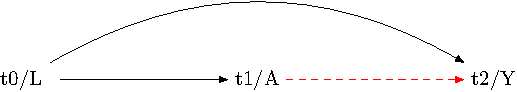
\includegraphics[width=0.8\textwidth,height=\textheight]{causal-dags_files/figure-pdf/fig-dag-common-cause-1.pdf}

}

\caption{\label{fig-dag-common-cause}Counfounding by common cause. The
dashed red arrow indicates bias arising from the open backdoor path from
A to Y.}

\end{figure}

\hypertarget{advice-attend-to-the-temporal-order-of-cauasality}{%
\subsection{Advice: attend to the temporal order of
cauasality}\label{advice-attend-to-the-temporal-order-of-cauasality}}

Confounding by a common cause can be addressed by adjusting for it.
Adjustment closes the backdoor path from the exposure to the outcome.
Typically we adjust through through statistical models such as
regression, matching, inverse probability of treatment weighting, and
G-methods. (Again, it is beyond the scope of this tutorial to describe
causal estimation techniques.) Figure
Figure~\ref{fig-dag-common-cause-solution} clarifies that any
confounding that is a cause of \(A\) and \(Y\) will precede \(A\) (and
so \(Y\)), because causes precede effects. By indexing the the nodes on
the graph, we can readily understand that \textbf{confounding control
typically requires time-series data.}

\begin{figure}

{\centering 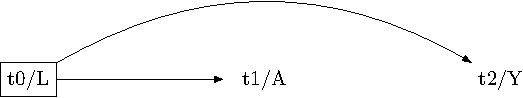
\includegraphics[width=0.8\textwidth,height=\textheight]{causal-dags_files/figure-pdf/fig-dag-common-cause-solution-1.pdf}

}

\caption{\label{fig-dag-common-cause-solution}Solution: adjust for
pre-exposure confounder.}

\end{figure}

\hypertarget{confounding-by-collider-stratification-conditioning-on-a-common-effect}{%
\subsection{2. Confounding by collider stratification (conditioning on a
common
effect)}\label{confounding-by-collider-stratification-conditioning-on-a-common-effect}}

Conditioning on a common effect occurs when a variable \(L\) is affected
by both the treatment \(A\) and an outcome \(Y\).

Suppose \(A\) and \(Y\) are initially independent, such that
\(A \coprod Y(a)\). Conditioning on the common effect \(L\) opens a
backdoor path between \(A\) and \(Y\), potentially inducing an
association. This occurs because \(L\) can provide information about
both \(A\) and \(Y\). Here is an example:

Let \(A\) denote the level of belief in Big Gods (with higher values
indicating stronger belief), \(Y\) denote the level of social
complexity, and \(L\) denote the level of economic trade. Now, suppose
that belief in Big Gods and social complexity are not causally linked.
However, both of these factors influence the level of economic trade,
and if we condition on economic trade in a cross-sectional study, we
might find a statistical association between belief in Big Gods and
social complexity even though there's no causal link.

If we denote the observed associations as follows:

\begin{itemize}
\tightlist
\item
  \(P(A)\): Distribution of beliefs in Big Gods
\item
  \(P(Y)\): Distribution of social complexity
\item
  \(P(L)\): Distribution of economic trade
\end{itemize}

Without conditioning on \(L\), and if \(A\) and \(Y\) are independent,
we have:

\[P(A, Y) = P(A)P(Y)\]

However, if we condition on \(L\) (which is a common effect of both
\(A\) and \(Y\)), we have:

\[P(A, Y | L) \neq P(A | L)P(Y | L)\]

The common effect \(L\), once conditioned on, creates an association
between \(A\) and \(Y\) that is not causal. This can mislead us into
believing there is a direct link between beliefs in Big Gods and social
complexity, even in the absence of such a link. If we only observe
\(A\), \(Y\), and \(L\) and compute correlations, without time-series
data measured on the units of analysis, we might erroneously conclude
that there is a causal relationship between \(A\) and \(Y\). This is an
example of collider-stratification bias, which occurs when we condition
on a common effect (a `collider') of two variables.\footnote{When \(A\)
  and \(Y\) are independent, the joint probability of \(A\) and \(Y\) is
  equal to the product of their individual probabilities:
  \(P(A, Y) = P(A)P(Y)\). However, when we condition on \(L\), the joint
  probability of \(A\) and \(Y\) given \(L\) is not necessarily equal to
  the product of the individual probabilities of \(A\) and \(Y\) given
  \(L\), hence the inequality \(P(A, Y | L) \neq P(A | L)P(Y | L)\).}

Conditioning on a common effect is an example of ``collider'' bias.

\begin{figure}

{\centering 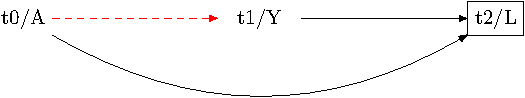
\includegraphics[width=0.8\textwidth,height=\textheight]{causal-dags_files/figure-pdf/fig-dag-common-effect-1.pdf}

}

\caption{\label{fig-dag-common-effect}Confounding by conditioning on a
collider. The dashed red arrow indicates bias arising from the open
backdoor path from A to Y.}

\end{figure}

\hypertarget{advice-attend-to-the-temporal-order-of-cauasality-and-show-this-in-your-causal-graph}{%
\subsection{Advice: attend to the temporal order of cauasality, and show
this in your causal
graph}\label{advice-attend-to-the-temporal-order-of-cauasality-and-show-this-in-your-causal-graph}}

To address the problem of conditioning on a common effect, we should
generally ensure that all confounders \(L\) that are common causes of
the exposure \(A\) and the outcome \(Y\) are measured before the
occurence of the exposure \(A\), and furthermore that the exposure \(A\)
is measured before the occurence of the outcome \(Y\). If such temporal
order is preserved, \(L\) cannot be an effect of \(A\), and thus neither
of \(Y\). By measuring all relevant confounders before the exposure,
researchers can minimise the scope for collider confounding by
conditioning on a common effect. This rule is not absolute.\footnote{However,
  as indicated in Figure~\ref{fig-dag-descendent-solution}, it may be
  useful in certain circumstances to condition on a confounder that
  occurs after the outcome has occurred.}. In the case of the example
just described, we would require time-series data with accurate measures
in a sufficiently large sample of cultures prior to the introduction of
certain religious beliefs, and the cultures would need to be independent
of each other.\footnote{The independence of cultural units was at the
  centre of the study of comparative urban archeaology throughout from
  the late 19th (\protect\hyperlink{ref-decoulanges1903}{De Coulanges
  1903}) and 20th century (\protect\hyperlink{ref-wheatley1971}{Wheatley
  1971}). Despite attention to this problem in recent work (e.g.
  (\protect\hyperlink{ref-watts2016}{Watts et al. 2016})), there is
  arguably greater ``head-room'' for understanding the need for
  conditional independence in recent cultural evolutionary studies.}

\begin{figure}

{\centering 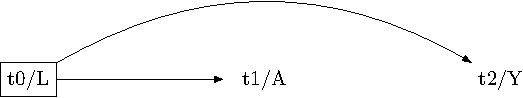
\includegraphics[width=0.8\textwidth,height=\textheight]{causal-dags_files/figure-pdf/fig-dag-common-effect-solution-1.pdf}

}

\caption{\label{fig-dag-common-effect-solution}Solution: time idexing of
confounders helps to avoid collider bias and maintain d-separation.}

\end{figure}

\hypertarget{m-bias-conditioning-on-a-collider-that-occurs-before-the-exposure-may-introduce-bias}{%
\subsection{M-bias: conditioning on a collider that occurs before the
exposure may introduce
bias}\label{m-bias-conditioning-on-a-collider-that-occurs-before-the-exposure-may-introduce-bias}}

Typically (with exceptions described below), indicators for confounders
should included only if they are known to be measured before their
exposures. However, researchers should be also cautious about
over-conditioning on pre-exposure variables that are not associated with
both the exposure and confounder, as doing so can induce confounding. As
shown in Figure~\ref{fig-m-bias}, collider stratification may arise even
if \(L\) occurs before \(A\). This happens when \(L\) does not affect
\(A\) or \(Y\), but may be the descendent of a unmeasured variable that
affects \(A\) and another unmeasured variable that also affects \(Y\).
Conditioning on \(L\) in this scenario evokes what is called ``M-bias.''
If \(L\) is not a common cause of both \(A\) and \(Y\), or the effect of
a shared common cause, \(L\) should not be included in a causal model.
Figure~\ref{fig-m-bias} presents a case in which \(A \coprod Y(a)\) but
\(A \cancel{\coprod} Y(a)| L\). M-bias is another example of collider
bias (see: (\protect\hyperlink{ref-cole2010}{Cole et al. 2010}))

\begin{figure}

{\centering 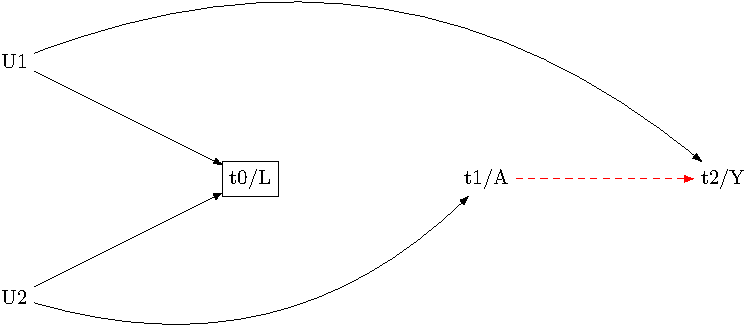
\includegraphics[width=0.8\textwidth,height=\textheight]{causal-dags_files/figure-pdf/fig-m-bias-1.pdf}

}

\caption{\label{fig-m-bias}M-bias: confounding control by including
previous measures of the outcome. The dashed red arrow indicates bias
arising from the open backdoor path from A to Y by conditioning on
pre-exposure variable L. The solution: do not condition on L.}

\end{figure}

\hypertarget{advice-adopt-a-modified-disjunctive-cause-criterion-for-confounding-control}{%
\subsection{Advice: adopt a modified disjunctive cause criterion for
confounding
control}\label{advice-adopt-a-modified-disjunctive-cause-criterion-for-confounding-control}}

Again, the modified disjunctive cause criterion will satisfy the
backdoor criterion in all cases, and reduce bias where this criterion
cannot be fully satisfied:

\begin{quote}
Control for each covariate that is a cause of the exposure, or of the
outcome, or of both; exclude from this set any variable known to be an
instrumental variable; and include as a covariate any proxy for an
unmeasured variable that is a common cause of both the exposure and the
outcome, see Tyler J. VanderWeele, Mathur, and Chen
(\protect\hyperlink{ref-vanderweele2020}{2020}) page 441 and
(\protect\hyperlink{ref-vanderweele2019a}{Tyler J. VanderWeele 2019})
\end{quote}

Of course, the difficulty is in determining which variables belong to
the desired set. This task can be facilitated by specialist knowledge
but cannot generally be ascertained from the data.

\hypertarget{the-problem-of-conditioning-on-a-mediator}{%
\subsection{3 The problem of conditioning on a
mediator}\label{the-problem-of-conditioning-on-a-mediator}}

Conditioning on a mediator occurs when \(L\) lies on the causal pathway
between the treatment \(A\) and the outcome \(Y\). Conditioning on \(L\)
can lead to biased estimates by blocking or distorting the total effect
of \(A\) and \(Y\).

Let \(A\) denote ``beliefs in Big Gods'', \(Y\) denote ``social
complexity'', and \(L\) denote ``economic trade''. Suppose that
``beliefs in Big Gods'' directly influences ``economic trade'', and
``economic trade'' in turn influences ``social complexity''. Here, \(L\)
(``economic trade'') acts as a mediator for the effect of \(A\)
(``beliefs in Big Gods'') on \(Y\) (``social complexity'').

If we condition on \(L\) (``economic trade''), we could potentially bias
our estimates of the total effect of \(A\) (``beliefs in Big Gods'') on
\(Y\) (``social complexity''). This is because conditioning on \(L\)
will typically attenuate the direct effect of \(A\) on \(Y\) as it
``blocks'' the indirect path through \(L\), as presented in
Figure~\ref{fig-dag-mediator}.

In the example just considered we do not induce bias under the null. If
\(A\) were not associated with \(Y\) then conditioning on \(M\) would
not open a backdoor path between \(A\) and \(L\). However, it is not
generally the case that conditioning on a mediator will not induce bias
under the null. As described below in Figure~\ref{fig-dag-descendent},
if \(L\) is the common effect of the exposure \(A\) and an unmeasured
variable \(U\) that is associated with the outcome \(Y\), then including
\(L\) may increase the strength of association between \(A\) and \(Y\),
even if \(A\) is not associated with \(Y\) and even if \(U\) is not a
cause of \(A\).

Therefore, unless one is interested in mediation analysis, conditioning
on a post-treatment variable is nearly always a bad idea (see
Figure~\ref{fig-dag-descendent-solution-2} for a counter example). Again
attention to chronology in the graph has practical implications for data
collection. If we cannot ensure that \(L\) is measured before \(A\) and
if \(A\) may affect \(L\), including \(L\) in our model risks mediator
bias.

\begin{figure}

{\centering 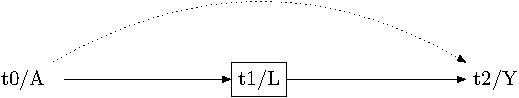
\includegraphics[width=0.8\textwidth,height=\textheight]{causal-dags_files/figure-pdf/fig-dag-mediator-1.pdf}

}

\caption{\label{fig-dag-mediator}Confounding by conditioning on a
mediator. The dashed black arrow indicates bias arising from partially
blocking the path between A and Y.}

\end{figure}

\hypertarget{advice-attend-to-the-temporal-order-of-causality}{%
\subsection{Advice: attend to the temporal order of
causality}\label{advice-attend-to-the-temporal-order-of-causality}}

To mitigate the issue of mediator bias, particularly when our focus is
on total effects, we should avoid conditioning on a mediator. This can
be achieved by ensuring that the mediator \(L\) takes place before the
treatment \(A\) and the outcome \(Y\). This underlines the importance of
explicitly stating the temporal ordering of our variables. By including
time indexing of all variables in our causal graph and by clearly
labelling mediators (e.g.~with \(M_t\)), we reduce the potential for
mediator bias from over-conditioning.\footnote{Note that if \(L\) is
  associated with \(Y\) and cannot be caused by \(A\), conditioning on
  \(L\) will often enhance the precision of the estimate for the causal
  effect of \(A\) on \(Y\). This holds true even if \(L\) occurs after
  \(A\). However, the onus is on us to explain that the post-treatment
  factor cannot be a consequence of the exposure. Moreover including
  \(L\) is not, in this instance, required for confounding control. We
  consider post-treatment conditioning next.}

\begin{figure}

{\centering 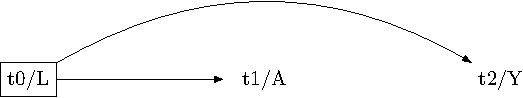
\includegraphics[width=0.8\textwidth,height=\textheight]{causal-dags_files/figure-pdf/fig-dag-mediator-solution-1.pdf}

}

\caption{\label{fig-dag-mediator-solution}Unless certain the exposure
cannot affect the confounder, ensure confounders are measured prior to
the exposure.}

\end{figure}

\hypertarget{conditioning-on-a-descendant}{%
\subsection{4. Conditioning on a
descendant}\label{conditioning-on-a-descendant}}

Say \(L\) is a cause of \(L^\prime\). According to Markov factorisation,
if we condition on \(L\) we partially condition on \(L^\prime\).

There are both negative and positive implications for causal estimation
in real-world scenarios.

First the negative. Suppose there is a confounder \(L^\prime\) that is
caused by an unobserved variable \(U\), and is affected by the treatment
\(A\). Suppose further that \(U\) causes the outcome \(Y\). In this
scenario, as described in Figure~\ref{fig-dag-descendent}, conditioning
on \(L^\prime\), which is a descendant of \(A\) and \(U\), can lead to a
spurious association between \(A\) and \(Y\) through the path
\(A \to L^\prime \to U \to Y\).

\begin{figure}

{\centering 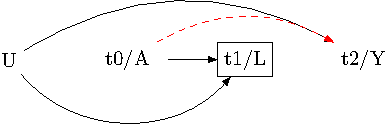
\includegraphics[width=0.8\textwidth,height=\textheight]{causal-dags_files/figure-pdf/fig-dag-descendent-1.pdf}

}

\caption{\label{fig-dag-descendent}Confounding by Descent: The red
dashed arrow illustrates the introduction of bias due to the opening of
a `backdoor' path between the exposure (A) and the outcome (Y) when
conditioning on a descendant of a confounder. This failure to maintain
d-separation in the association between the exposure and the outcome
leads to potential bias in the causal inference.}

\end{figure}

\hypertarget{advice-attend-to-the-temporal-order-of-causality-and-use-expert-knowledge-of-all-relevant-nodes.}{%
\subsection{Advice: attend to the temporal order of causality, and use
expert knowledge of all relevant
nodes.}\label{advice-attend-to-the-temporal-order-of-causality-and-use-expert-knowledge-of-all-relevant-nodes.}}

Ensuring the confounder (\(L^\prime\)) is measured before the exposure
(\(A\)) has two benefits.

First, if \(L^\prime\) is a confounder, that is, if \(L^\prime\) is a
variable which if we fail to condition on it will bias the association
between treatment and outcome, the strategy of including only
pre-treatment indicators of \(L\prime\) will reduce bias.
Figure~\ref{fig-dag-descendent-solution} presents this strategy

\begin{figure}

{\centering 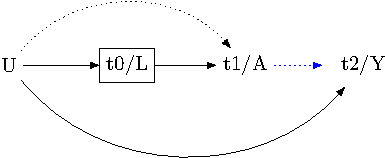
\includegraphics[width=0.8\textwidth,height=\textheight]{causal-dags_files/figure-pdf/fig-dag-descendent-solution-1.pdf}

}

\caption{\label{fig-dag-descendent-solution}Solution: again, ensure
temporal ordering in all measured variables. A and Y remain
d-separated.}

\end{figure}

Second, note that we may use descendent to reduce bias. For example, if
an unmeasured confounder \(U\) affects \(A\), \(Y\), and \(L^\prime\),
then adjusting for \(L^\prime\) may help to reduce confounding caused by
\(U\). This scenario is presented in
Figure~\ref{fig-dag-descendent-solution-2}, and clarifies why the the
modified disjunctive cause criterion for confounding control advises
that we ``include as a covariate any proxy for an unmeasured variable
that is a common cause of both the exposure and the outcome''
(\protect\hyperlink{ref-vanderweele2019a}{Tyler J. VanderWeele 2019}).

Note furthermore that in this graph, \(L^\prime\) may occur \emph{after}
the exposure, and indeed occurs \emph{after} the outcome. This shows
that it would be wrong to infer that merely because causes precede
effects, we should only condition on confounders that precede the
exposure.

\begin{figure}

{\centering 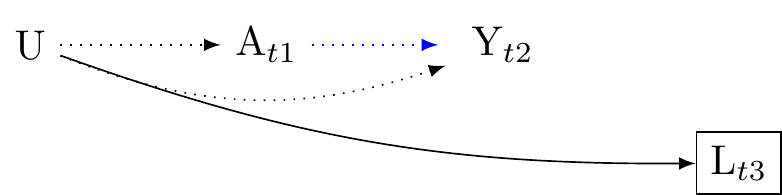
\includegraphics[width=0.8\textwidth,height=\textheight]{causal-dags_files/figure-pdf/fig-dag-descendent-solution-2-1.pdf}

}

\caption{\label{fig-dag-descendent-solution-2}Solution: conditioning on
a confounder that occurs after the exposure and the outcome may address
a problem of unmeasured confounding if the confounder is a descendent of
a prior common cause of the exposure and outcome. The dotted paths
denote that the effect of U on A and Y is partially adjusted by
conditioning on L', even though L' occurs after the outcome. The dotted
blue represents suppressing bias. For example a genetic factor that
affects the exposure and the outcome early in life might be measured by
an indicator late that is expressed (and may be measured) later in life.
Adjusting for such and indicator would constitute an example of
post-outcome confounding control.}

\end{figure}

\hypertarget{case-1-causal-interaction-do-not-attempt-to-draw-non-linear-relationships-such-as-interactions}{%
\subsection{Case 1: causal Interaction: do not attempt to draw
non-linear relationships such as
interactions}\label{case-1-causal-interaction-do-not-attempt-to-draw-non-linear-relationships-such-as-interactions}}

Those studying causal diagramms often wonder how to depict interactions
within these structures. This is a sensible question, especially because
interactions can be scientifically important. However, it is crucial to
remember the primary function of causal diagramms: to ensure
d-separation (conditional independence) between exposure and outcome
variables. Causal diagrams are not designed to capture all facets of a
phenomenon under investigation. Furthermore, causal diagrams are
qualitative tools and do not inherently represent non-parametric
characteristics of reality, such as additive and multiplicative
interaction.

Some misunderstandings can arise regarding the role and function of
causal diagrams. These often stem from deeper confusions about the
concept of interaction itself. Given this, it is worth taking a moment
to clarify the notion of interaction within a counterfactual causal
framework. Again, in much scientific research, evaluating evidence for
interaction is oftent important. However, to accurately handle this
concept, a crucial distinction must be made between causal interaction
and effect modification.

\hypertarget{causal-interaction-as-two-independent-exposures-what-to-graph}{%
\subsubsection{\texorpdfstring{\textbf{Causal interaction as two
independent exposures: what to
graph}}{Causal interaction as two independent exposures: what to graph}}\label{causal-interaction-as-two-independent-exposures-what-to-graph}}

Causal interaction is the effect of two exposures that may occur jointly
or separately (or not occur). We say there is interaction on the scale
of interest when the effect of one exposure on an outcome depends on the
level of another exposure. For example, the effect of a beliefs in Big
Gods (exposure A) on social complexity (outcome Y) might depend on
whether a culture has monumental architecture (exposure B), which in
turn might also affect social complexity. Evidence for causal
interaction on the difference scale would be present if:

\[\bigg(\underbrace{E[Y(1,1)]}_{\text{joint exposure}} - \underbrace{E[Y(0,0)]}_{\text{neither exposed}}\bigg) - \bigg[ \bigg(\underbrace{E[Y(1,0)]}_{\text{only A exposed}} - \underbrace{E[Y(0,0)]}_{\text{neither exposed}}\bigg) + \bigg(\underbrace{E[Y(0,1)]}_{\text{only B exposed}} - \underbrace{E[Y(0,0)]}_{\text{neither exposed}} \bigg)\bigg] \neq 0 \]

This simplifies to:

\[ \underbrace{E[Y(1,1)]}_{\text{joint exposure}} - \underbrace{E[Y(1,0)]}_{\text{only A exposed}} - \underbrace{E[Y(0,1)]}_{\text{only B exposed}} + \underbrace{E[Y(0,0)]}_{\text{neither exposed}} \neq 0 \]

If these equations hold, the effect of exposure A on the outcome is not
the same across different levels of exposure B, or vice versa,
indicating there is an interaction between exposure A and exposure B.

If the quantity on the left hand side is greater than zero there is
evidence for positive interaction; if it is less than zero there is
evidence a sub-additive effect; if this quantity is indistinguishable
from zero we say there is no evidence for interaction.\footnote{Note
  that the causal effects of interactions often differ when measured on
  the ratio scale. This can have important policy implications, see:
  (\protect\hyperlink{ref-vanderweele2014}{Tyler J. VanderWeele and Knol
  2014}). Although beyond the scope of this article, when evaluating
  evidence for causality we must clarify the measure of effect in which
  we are interested(\protect\hyperlink{ref-hernuxe1n2004}{M. A. Hernán
  2004}; \protect\hyperlink{ref-tripepi2007}{Tripepi et al. 2007}).}

How do we represent interaction on a causal graph? Remember, causal
diagrams are not parametric; they represent the qualitative aspects of
causal relationships without making specific assumptions about the
functional form of these relationships. We do not use causal diagrams to
represent interactions. We use them to identify sources of confounding
and strategies for confounding control. Although causal diagrams can
indicate the presence of an interaction by showing two exposures jointly
influencing an outcome, as in Figure~\ref{fig-dag-interaction}, they do
not represent the nature or scale of the interaction directly.

\begin{figure}

{\centering 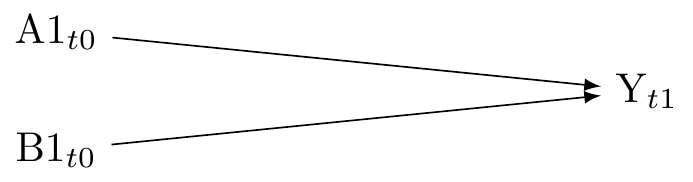
\includegraphics[width=0.4\textwidth,height=\textheight]{causal-dags_files/figure-pdf/fig-dag-interaction-1.pdf}

}

\caption{\label{fig-dag-interaction}Causal interaction: if two exposures
are causally independent of each other, we may wish to estimate their
individual and joint effects on Y, where the counterfactual outcome is
Y(a,b) and there is evidence for additive or subadditive interaction if
E{[}Y(1,1) - Y(0,1) - Y(1,0) + Y(0,0){]} ≠ 0. If we cannot conceptualise
B as a variable upon which there can be intervention, then the
interaction is better conceived as effect modification (see next
figure). Important: DAGs are not parametric so to express interaction do
not draw a path into another path, or attempt other such shenanigans.}

\end{figure}

\hypertarget{causal-interaction-considered-as-effect-modification-what-to-graph}{%
\subsubsection{\texorpdfstring{\textbf{Causal interaction considered as
effect modification: what to
graph}}{Causal interaction considered as effect modification: what to graph}}\label{causal-interaction-considered-as-effect-modification-what-to-graph}}

When discussing evidence for effect modification, we're essentially
looking at how the effect of a given exposure on an outcome varies
according to different levels of another variable. For instance,
consider a study where we're interested in how the influence of belief
in Big Gods on social complexity might vary between early urban
civilizations in China and South America. In this scenario, `geography'
(China versus South America) serves as the `effect modifier.' That is,
to investigate effect modification, we focus on how the influence of our
exposure (belief in Big Gods) on the outcome (social complexity) differs
across various levels of our effect modifier (geography). It is
important to note that we are not considering the effect modifier as a
variable on which we intervene, but merely one that might change the
effect of our exposure on the outcome of interest.

To fill this out, suppose we are comparing two levels of exposure, which
we'll call \(A = a\) and \(A= a^*\). Suppose further that \(G\) has two
levels, which we will call \(g\) and \(g'\). Then:

\[\hat{E}[Y(a)|G=g]\]

represents the expected outcome when the exposure is at level \(A=a\)
among individuals in group \(G=g\).

\[\hat{E}[Y(a^*)|G=g]\]

represents the expected outcome when the exposure is at level \(A=a^*\)
among individuals in group \(G=g\).

The difference

\[\hat{\delta}_g = \hat{E}[Y(a)|G=g] - \hat{E}[Y(a^*)|G=g]\]

is our estimated causal effect of changing the exposure from \(a^*\) to
\(a\) in group \(g\).

Similarly,
\[\hat{\delta}_{g'} = \hat{E}[Y(a)|G=g'] - \hat{E}[Y(a^*)|G=g']\] is our
estimated causal effect of changing the exposure from \(a^*\) to \(a\)
in group \(g'\).

Finally, we can compare the causal effects between these two groups by
computing

\[\hat{\gamma} = \hat{\delta}_g - \hat{\delta}_{g'}\]

This value, \(\hat{\gamma}\), tells us how much the impact of changing
the exposure from \(a^*\) to \(a\) varies between groups \(g\) and
\(g'\). If \(\hat{\gamma}\neq 0\) this implies that the exposure has a
different effect in the two groups, indicating effect modification.

When representing effect modification, it is again important to remember
that causal diagrams are not parametric. Thus to represent effect
modification, do \emph{not} draw a path intersecting another path or
attempt another visualisation. Rather, simply draw two edges into to
exposure Figure~\ref{fig-dag-effect-modfication}. Keep at the front of
your mind that your purpose in drawing a causal graph is to assess
confoundings and to addressing the identification problem. Here again,
representing the temporal order of events in the spatial layout of your
graph will make the identification problem clearer because causes must
precede effects.(To understand finer-grained distinctions see:
(\protect\hyperlink{ref-vanderweele2007}{Tyler J. VanderWeele and Robins
2007}).)

\begin{figure}

{\centering 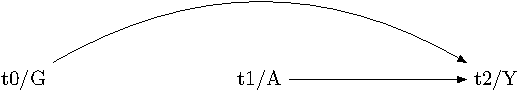
\includegraphics[width=0.8\textwidth,height=\textheight]{causal-dags_files/figure-pdf/fig-dag-effect-modfication-1.pdf}

}

\caption{\label{fig-dag-effect-modfication}A simple graph for
effect-modification.}

\end{figure}

\hypertarget{case-2-causal-mediation-causal-graphs-show-the-inadequacy-of-standard-approaches}{%
\subsection{Case 2: Causal mediation: causal graphs show the inadequacy
of standard
approaches}\label{case-2-causal-mediation-causal-graphs-show-the-inadequacy-of-standard-approaches}}

The conditions necessary for causal mediation are stringent.
Chronologically arranged causal diagrams, as shown in
Figure~\ref{fig-dag-mediation-assumptions}, can aid us in identifying
both the promise and perils of causal mediation. We will again keep to
the question of whether cultural beliefs in Big Gods affect social
complexity, and ask whether this affect is mediated by political
authority.

\begin{enumerate}
\def\labelenumi{\arabic{enumi}.}
\tightlist
\item
  \textbf{No unmeasured exposure-outcome confounders given} \(L\)
\end{enumerate}

This prerequisite is expressed as \(Y(a,m) \coprod A | L1\). Upon
controlling for the covariate set \(L1\), we must ensure that there are
no additional unmeasured confounders affecting both the cultural beliefs
in Big Gods \(A\) and the social complexity \(Y\). For example, if our
study involves the impact of cultural beliefs in Big Gods (exposure) on
social complexity (outcome), and geographic location and historical
context are our covariates \(L1\), this assumption of no unmeasured
confounding suggests that accounting for \(L1\) sufficiently covers any
subsequent correlation between \(A\) and \(Y\). The relevant confounding
path is depicted in brown in Figure~\ref{fig-dag-mediation-assumptions}.

\begin{enumerate}
\def\labelenumi{\arabic{enumi}.}
\setcounter{enumi}{1}
\tightlist
\item
  \textbf{No unmeasured mediator-outcome confounders given} \(L\)
\end{enumerate}

This condition is expressed as \(Y(a,m) \coprod M | L2\). Upon
controlling for the covariate set \(L2\), we must ensure that no other
unmeasured confounders affect both the political authority \(M\) and
social complexity \(Y\). For instance, if trade networks impact both
political authority and social complexity, we must account for trade
networks to obstruct the otherwise unblocked path linking our mediator
and outcome. Further, we must assume the absence of any other
confounders for the mediator-outcome path. This confounding path is
represented in blue in Figure~\ref{fig-dag-mediation-assumptions}.

\begin{enumerate}
\def\labelenumi{\arabic{enumi}.}
\setcounter{enumi}{2}
\tightlist
\item
  \textbf{No unmeasured exposure-mediator confounders given} \(L\)
\end{enumerate}

This requirement is represented as \(M(a) \coprod A | L3\). Upon
controlling for the covariate set \(L3\), we must ensure that there are
no additional unmeasured confounders affecting both the cultural beliefs
in Big Gods \(A\) and political authority \(M\). For example, the
capability to construct large ritual theaters may influence both the
belief in Big Gods and the level of political authority. If we have
indicators for this technology measured prior to the emergence of Big
Gods (these indicators being \(L3\)), we must assume that accounting for
\(L3\) is enough to obstruct the backdoor path between the exposure and
the mediator for unbiased natural mediated effect estimation. This
confounding path is shown in green in
Figure~\ref{fig-dag-mediation-assumptions}.

\begin{enumerate}
\def\labelenumi{\arabic{enumi}.}
\setcounter{enumi}{3}
\tightlist
\item
  \textbf{No mediator-outcome confounder affected by the exposure (no
  red arrow)}
\end{enumerate}

This requirement is indicated as \(Y(a,m) \coprod M^{a^*} | L\). We must
ensure that no variables confounding the relationship between political
authority and social complexity in \(L2\) are themselves influenced by
the cultural beliefs in Big Gods (\(A\)). For instance, when studying
the effect of cultural beliefs in Big Gods (\(A\), the exposure) on
social complexity (\(Y\), the outcome) mediated by political authority
(mediator), this assumption means that there are no factors, such as
trade networks (\(L2\)), that influence both political authority and
social complexity and are affected by the belief in Big Gods. This
confounding path is shown in red in
Figure~\ref{fig-dag-mediation-assumptions}. It is important to note that
\textbf{the assumption of no mediator/outcome confounder affected by the
exposure is challenging to satisfy}. If the exposure influences a
confounder of the mediator and outcome, we face a dilemma. If we do not
account for this confounder, the backdoor path between the mediator and
outcome remains open. By accounting for it, however, we partially
obstruct the path between the exposure and mediator, leading to bias.
Consequently, the natural direct and indirect effects can't be
identified from the manifest data, even with perfect measures of the
relevant confounders. Notice again that the requirements for
counterfactual data science are more strict than for descriptive or
predictive data science. Nonetheless, we can set the mediator to certain
levels and explore controlled direct and indirect effects, which may be
relevant for science and policy. For instance, if we were to fix
political authority at a specific level, we could ask, what would be the
direct and indirect causal effects of Big Gods on Social Complexity?
There are other approaches that involve sampling from the observed
distributions to obtain probablistic identification (an excellent
resource is (\protect\hyperlink{ref-shi2021}{Shi et al. 2021}) ).
Answering such questions typically necessitates the use of G-methods,
which the subsequent section will elaborate on. For now, we have seen
how chronologically ordered causal diagrams elucidate the conditions
necessary for mediation analysis in addressing causal
questions.\footnote{An excellent resource both for understanding causal
  interaction and causal mediation is
  (\protect\hyperlink{ref-vanderweele2015a}{T. VanderWeele 2015b}).}

\begin{figure}

{\centering \includegraphics[width=0.8\textwidth,height=\textheight]{causal-dags_files/figure-pdf/fig-dag-mediation-assumptions-1.pdf}

}

\caption{\label{fig-dag-mediation-assumptions}Assumptions for mediation
analysis. The brown edges denote the path for common causes of the
exposure and coutcome. To block this path we must condition on L1. The
green edges denote the path for common causes of the exposure and
mediator. To block this path we must condition on L3. The blue edges
denote the path for common causes of the mediator and outcome. To block
this path we must condition on L2. The red path denotes the effect of
the exposure on the confounder of the mediator and outcome. If any such
path exists then we cannot obtain natural direct and indirect effects.
Conditioning on L2 is necessary to prevent mediator outcome confounding
but doing so blocks the effect of the exposure on the mediator.}

\end{figure}

\hypertarget{case-3-confounder-treatment-feedback-causal-graphs-show-the-inadequacy-of-standard-approaches}{%
\subsection{Case 3: Confounder-treatment feedback: causal graphs show
the inadequacy of standard
approaches}\label{case-3-confounder-treatment-feedback-causal-graphs-show-the-inadequacy-of-standard-approaches}}

Causal mediation is a special case in which we have multiple sequential
exposures. Here again chronologically organised causal diagrams can help
us to understand the problems and opportunities for causal inference
using time-series data.

For example, consider temporally fixed multiple exposures. The
counterfactual outcomes may be denoted \(Y(a_{t1} ,a_{t2})\). There are
four counterfactual outcomes corresponding to the four fixed ``treatment
regimes'':

\begin{enumerate}
\def\labelenumi{\arabic{enumi}.}
\item
  \textbf{Always treat (Y(1,1))}: This regime involves providing the
  treatment at every opportunity.
\item
  \textbf{Never treat (Y(0,0))}: This regime involves abstaining from
  providing the treatment at any opportunity.
\item
  \textbf{Treat once first (Y(1,0))}: This regime involves providing the
  treatment only at the first opportunity and not at subsequent one.
\item
  \textbf{Treat once second (Y(0,1))}: This regime involves abstaining
  from providing the treatment at the first opportunity, but then
  providing it at the second one.
\end{enumerate}

There are six causal contrasts that we might compute for the four fixed
regimes, presented in \textbf{?@tbl-regimes}.\footnote{We compute the
  number of possible combinations of contrasts by
  \(C(n, r) = \frac{n!}{(n-r)! \cdot r!}\)}

\begin{longtable}[]{@{}
  >{\raggedright\arraybackslash}p{(\columnwidth - 4\tabcolsep) * \real{0.1351}}
  >{\raggedright\arraybackslash}p{(\columnwidth - 4\tabcolsep) * \real{0.5405}}
  >{\raggedright\arraybackslash}p{(\columnwidth - 4\tabcolsep) * \real{0.3243}}@{}}
\caption{Table describes four fixed treatment regimes and six causal
contrasts in time series data where the exposure may
vary.}\tabularnewline
\toprule\noalign{}
\begin{minipage}[b]{\linewidth}\raggedright
Type
\end{minipage} & \begin{minipage}[b]{\linewidth}\raggedright
Description
\end{minipage} & \begin{minipage}[b]{\linewidth}\raggedright
Counterfactual Outcome
\end{minipage} \\
\midrule\noalign{}
\endfirsthead
\toprule\noalign{}
\begin{minipage}[b]{\linewidth}\raggedright
Type
\end{minipage} & \begin{minipage}[b]{\linewidth}\raggedright
Description
\end{minipage} & \begin{minipage}[b]{\linewidth}\raggedright
Counterfactual Outcome
\end{minipage} \\
\midrule\noalign{}
\endhead
\bottomrule\noalign{}
\endlastfoot
Regime & Always treat & Y(1,1) \\
Regime & Never treat & Y(0,0) \\
Regime & Treat once first & Y(1,0) \\
Regime & Treat once second & Y(0,1) \\
Contrast & Always treat vs.~Never treat & E{[}Y(1,1) - Y(0,0){]} \\
Contrast & Always treat vs.~Treat once first & E{[}Y(1,1) - Y(1,0){]} \\
Contrast & Always treat vs.~Treat once second & E{[}Y(1,1) -
Y(0,1){]} \\
Contrast & Never treat vs.~Treat once first & E{[}Y(0,0) - Y(1,0){]} \\
Contrast & Never treat vs.~Treat once second & E{[}Y(0,0) - Y(0,1){]} \\
Contrast & Treat once first vs.~Treat once second & E{[}Y(1,0) -
Y(0,1){]} \\
\end{longtable}

We might also consider treatment to be a function of the previous
outcome. For example, we might \textbf{Treat once first} and then
\textbf{treat again} or \textbf{do not treat again} depending on the
outcome of the previous treatment. This is called ``time-varying
treatment regimes.''

Note that to estimate the ``effect'' of a treatment regime, we must
compare the counterfactual quantities of interest. The same conditions
that apply for causal identification in mediation analysis apply to
causal identification in multiple treatment settings. And notice, just
as mediation opens the possibility of time-varying confounding
(condition 4, in which the exposure effects the confounders of the
mediator/outcome path), so too we find that with time-varying treatments
comes the problem of time-varying confounding. Unlike traditional causal
mediation analysis, the sequence of treatment regimes that we might
consider is indefinitely long.

Temporally organised causal diagrams again help us to discover the
problems with traditional multi-level regression analysis and structural
equation modelling. Suppose we are interested in the question of whether
beliefs in big Gods affect social complexity.

First consider fixed regimes. Suppose we have well-defined concept of
social complexity and excellent measurements over time. Suppose we want
to compare the effects of beliefs on big Gods on Social complexity using
historical data measured over two centuries. Our question is whether the
introduction and persistence of such beliefs differs from having no such
beliefs. The treatment strategies are: ``always believe in big Gods''
versus ``never believe in big Gods'' on the level of social complexity.
Consider Figure~\ref{fig-dag-9}. Here, \(A_{tx}\) represents the
cultural belief in ``Big Gods'' at time \(tx\), and \(Y_{tx}\) is the
outcome, social complexity, at time \(x\). Economic trade, denoted as
\(L_{tx}\), is a time-varying confounder because it varies over time and
confounds the effect of \(A\) on \(Y\) at several time points \(x\). To
complete our causal diagramme we include an unmeasured confounder \(U\),
such as oral traditions, which might influence both the belief in big
Gods and social complexity.

We know that the level of economic trade at time \(0\), \(L_{t0}\),
influences the belief in ``big Gods'' at time \(1\), \(A_{t1}\). We
therefore draw an arrow from \(L_{t0}\) to \(A_{t1}\). But we also know
that the belief in ``big Gods'', \(A_{t1}\), affects the future level of
economic trade, \(L_{t(2)}\). This means that we need to add an arrow
from \(A_{t1}\) to \(L_{t2}\). This causal graph represents a feedback
process between the time-varying exposure \(A\) and the time-varying
confounder \(L\). This is the simplest graph with exposure-confounder
feedback. In real world setting there would be more arrows. However, our
DAG need only show the minimum number of arrows to exhibit the problem
of exposure-confounder feedback. (We should not clutter our causal
diagrams: only provide the essential details.)

What happens if we were to condition on the time-varying confounder
\(L_{t3}\)? Two things would occur. First, we would block all the
backdoor paths between the exposure \(A_{t2}\) and the outcome. We need
to block those paths to eliminate confounding. Therefore, conditioning
on the time-varying confounding is essential. However, paths that were
previously blocked would not be pen. For example, the path
\(A_{t1}, L_{t2}, U, Y_{t(4)}\), which was previous closed is opened
because the time varying confounder is the common effect of \(A_{t1}\)
and \(U\). Conditioning opens the path \(A_{t1}, L_{t2}, U, Y_{3}\).
Therefore we must avoid conditioning on the time varying confounder. We
are damned-if-we-do-or-do-not condition on the confounder that is
affected by the prior exposure.

As with mediation, however, is may be possible to identify controlled
causal effects. Models for assessing such controlled causal effects of
time-fixed and time-varying exposures belong to a class of methods
called ``G-methods'' (\protect\hyperlink{ref-naimi2017}{Naimi, Cole, and
Kennedy 2017}; \protect\hyperlink{ref-chatton2020}{Chatton et al. 2020};
\protect\hyperlink{ref-robins}{Robins and Hernán, n.d.};
\protect\hyperlink{ref-hernuxe1n2006}{Miguel A. Hernán and Robins 2006})
There has been rapid recent development in the applications of G-methods
in the health sciences (\protect\hyperlink{ref-williams2021}{Williams
and Díaz 2021}; \protect\hyperlink{ref-duxedaz2021}{Díaz et al. 2021};
\protect\hyperlink{ref-breskin2021}{Breskin et al. 2021}). However,
G-methods have yet to be widely employed by cultural evolutionary
researchers. causal diagrams are important because they help to clarify
the fact that standard methods -- including multi-level regression
models -- will fail to recover natural causal effects from time-series
data in which there is treatment-confounder feedback.

\begin{figure}

{\centering 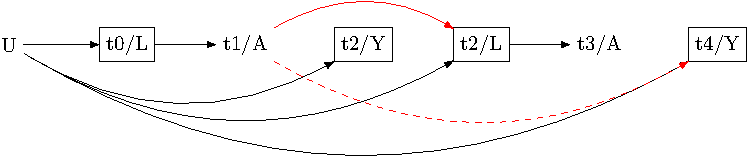
\includegraphics[width=1\textwidth,height=\textheight]{causal-dags_files/figure-pdf/fig-dag-9-1.pdf}

}

\caption{\label{fig-dag-9}Exposure confounder feedback is a problem for
time-series models. If we do not condition on L\_t2, a backdoor path is
open from A\_t3 to Y\_t4. However, if conditioning on L\_t2 introduces
collider bias, opening a path, coloured in red, between A\_t2 and Y\_t4.
Here, we may not use conventional methods to estimate the effects of
multiple exposures. Instead, at best, we may only simulate controlled
effects using G-methods. Multi-level models will eliminate bias.
Currently, outside of epidemiology, G-methods are rarely used. causal
diagrams are useful for clarifying the damned either way confounding
control strategies that lead traditional methods to fail.}

\end{figure}

A similar problem arises when the time-varying exposure and time-varying
confounder share a common cause. The problem arises even without the
exposure affecting the confounder.

\begin{figure}

{\centering 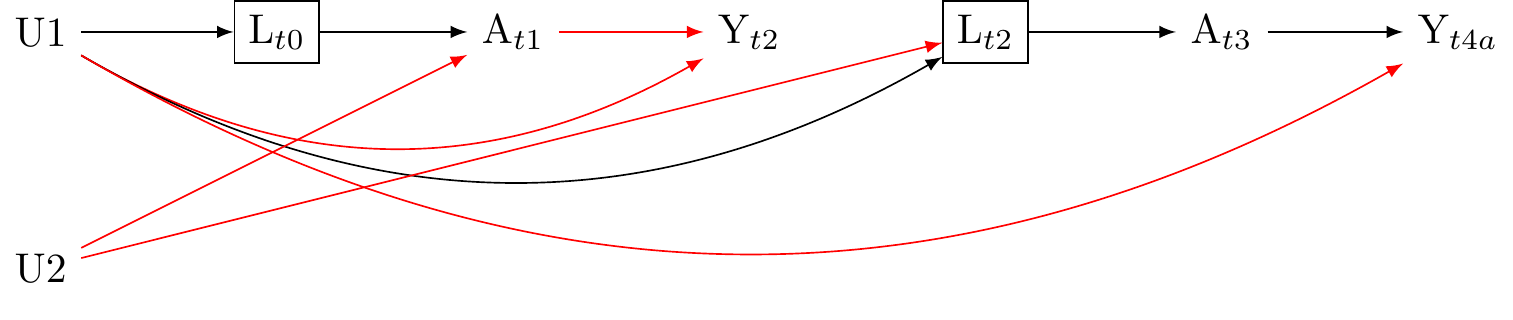
\includegraphics[width=1\textwidth,height=\textheight]{causal-dags_files/figure-pdf/fig-dag-time-vary-common-cause-A1-l1-1.pdf}

}

\caption{\label{fig-dag-time-vary-common-cause-A1-l1}Exposure confounder
feedback is a problem for time-series models. Here, the problem arises
from an unmeasured variable (U2) that affects both the exposure A at
time 1 and the counfounder L at time 2. The red paths show the back door
path that is opened when we condition on the L at time 2. Again, this
problem cannot be addressed with regression-based methods. In this
setting, to address causal questions, we may only use simulation based
G-methods. causal diagrams are useful in clarifying problems for
identifying causal effects from manifest data, even when the data are
large and perfectly measured.}

\end{figure}

The problem becomes accute when the exposures \(A_{t1}\) affects the
outcome \(Y_{t4}\). Consider: because \(L_{t2}\) is along the path from
\(A_{t1}\) to \(Y_{t4}\) conditioning on \(L_{t2}\) partially blocks the
path between the exposure and the outcome. Conditioning on \(L_{t2}\) in
this setting induces both collider stratification bias and mediator
bias. Yet we must condition on \(L_{t2}\) to block the open backdoor
path between \(L_{t2}\) and \(Y_{t4}\). The general problem of
exposure-confounder feedback is described in
(\protect\hyperlink{ref-hernan2023b}{Hernan and Robins 2023b}). This
problem presents a serious issue for cultural evolutionary studies. The
bad news is that nearly traditional regression based methods cannot
address this problem. Causality is not identified from time-series data
with feedback. The good news, again, is that we may obtain controlled
effect estimates in these settings using G-methods , where there have
been many recent developments. The scope and application of these
methods is beyond the scope of this tutorial.\footnote{Relatedly, to
  assess the identification of controlled effect estimates benefits from
  graphical methods such as ``single world intervention graphs'' or
  ``SWIGS.'' SWIGS represent counterfactual outcomes on the graph.
  However, in their general form, SWIGS are templates and not causal
  diagrams. Their application, too, is beyond the scope of this tutorial
  see: (\protect\hyperlink{ref-richardson2013}{Richardson and Robins
  2013})}

\hypertarget{summary-part-2}{%
\subsection{Summary Part 2}\label{summary-part-2}}

To estimate causal effects we must contrast the world as it has been
with the world as it might have been. For many big questions in cultural
evolution, we have seen confounder-treatment feedback leads to
intractable identification problems. We have also seen that causal
diagrams are useful for clarifying these problems. I next turn to
three-wave designs for estimating the total causal effects. Such designs
have applications for a broad class of cultural evolutionary questions,
and may be especially useful for evolutionary anthropologists who wish
to collect time-series data in the present to address causal questions
about cultural evolution as it is occurring in the world today.

\hypertarget{part-3.-applications-the-three-wave-panel-design.}{%
\section{Part 3. Applications: the three wave panel
design.}\label{part-3.-applications-the-three-wave-panel-design.}}

In this section, we explore how temporally ordered causal diagrams can
illuminate the utility of a three-wave panel design for addressing
causal questions using data as described by Tyler J. VanderWeele,
Mathur, and Chen (\protect\hyperlink{ref-vanderweele2020}{2020}). Here
is how we can address causal questions with three waves of data.

\hypertarget{step-1.-examine-the-utility-of-a-three-wave-panel-design-through-temporally-ordered-causal-diagram}{%
\subsection{Step 1. Examine the utility of a three-wave panel design
through temporally ordered causal
diagram}\label{step-1.-examine-the-utility-of-a-three-wave-panel-design-through-temporally-ordered-causal-diagram}}

In this section, we examine into how temporally ordered causal diagrams
can highlight the effectiveness of a three-wave panel design in
addressing causal questions, as elaborated by Tyler J. VanderWeele,
Mathur, and Chen (\protect\hyperlink{ref-vanderweele2020}{2020}).
Consider how to approach causal questions with three waves of data.

\hypertarget{step-2.-specify-the-exposure-and-measure-it-at-wave-0-and-wave-1.}{%
\subsection{Step 2. Specify the exposure and measure it at wave 0 and
wave
1.}\label{step-2.-specify-the-exposure-and-measure-it-at-wave-0-and-wave-1.}}

Initially, we need a well-defined exposure. Unless our interest is in
causal interaction, causal mediation, or sequential treatment regimes,
we will investigate the total effect of only one exposure. Suppose we
are interested in investigating the causal effect of religious service
attendance. Our first task is to explicitly state the the exposure as a
hypothetical intervention: Is our interest in any attendance versus
non-attendance?, weekly attendance versus monthly attendance? or some
other state. Imagining a hypothetical experiment, even if not feasible,
helps to focus on the need to state a clear intervention
(\protect\hyperlink{ref-hernuxe1n2022a}{Miguel A. Hernán, Wang, and Leaf
2022}).

In a three-wave panel design, we must measure the exposure both at
baseline and at the second wave. This dual measurement strategy plays a
crucial role in the effort to use observational data to replicate the
design of a controlled experiment. When an exposure is recorded at the
baseline and the second wave, we ensure that what we are assessing is
the effect of the ``incident exposure'' - an exposure newly occurring
between the first and second waves. This is distinct from the
``prevalent exposure,'' that is the frequency of the distribution of
exposure in the population at baseline
(\protect\hyperlink{ref-danaei2012}{Danaei, Tavakkoli, and Hernán 2012};
\protect\hyperlink{ref-hernan2023}{Hernan and Robins 2023a}). By
controlling for baseline exposure we more effectively emulate an
experimental manipulation of a factor of interest, wherein an
intervention is applied at a particular point in time and subsequent
changes are observed. Consider how biase might occur if the exposure is
initially harmful to the outcome. Suppose we only measure the exposure
at the second wave and ignore the initial exposure at baseline (see:
Figure~\ref{fig-dag-descendent-solution-2}.). In that case, we might
wrongly infer that the exposure is benefitial
(\protect\hyperlink{ref-hernuxe1n2008a}{Miguel A. Hernán et al. 2008};
\protect\hyperlink{ref-hernuxe1n2016a}{Miguel A. Hernán et al. 2016}).

An further advantage of controlling for the exposure at baseline is that
it can reduce the probability of bias that might arise if there is an
unmeasured confounder affecting both the outcome and the initial
exposure, irrespective of the previous exposure levels.

\hypertarget{caution-if-the-exposure-is-rare-large-amounts-of-data-must-be-collected-to-estimate-causal-effects}{%
\subsubsection{\texorpdfstring{\textbf{Caution: if the exposure is rare,
large amounts of data must be collected to estimate causal
effects}}{Caution: if the exposure is rare, large amounts of data must be collected to estimate causal effects}}\label{caution-if-the-exposure-is-rare-large-amounts-of-data-must-be-collected-to-estimate-causal-effects}}

Suppose that in the non religious population the switch from zero
religious service attendance to weekly religious service attendance
rarely: say 1 in 1,000 non attenders per year. To obtain an effective
sample for a ``treatment'' group while conditioning on a rich set of
might not be feasible without 100s of thousands of participants. One
might be better to consider change within the religious population,
assuming the change is more common in this population. However, in this
case, we would not generally estimate a causal effect that would
transport to the non-religious population. We would rather estimate a
causal effect that generalised to the religious population from which
the sample was drawn.

\hypertarget{step-3.-specify-the-outcomes-and-measure-them-at-wave-0-and-wave-2}{%
\subsection{Step 3. Specify the outcome(s) and measure them at wave 0
and wave
2}\label{step-3.-specify-the-outcomes-and-measure-them-at-wave-0-and-wave-2}}

After defining the exposure, we need a to state a well-defined outcome,
or outcomes. In our case, we might be interested in the effect of
gaining or losing religious beliefs on the frequency of volunteering
(e.g., weekly, monthly, yearly). Note that vague concepts such as ``the
societal effects of religious change'' do not lead us toward
understanding causality. We must specify what we mean by ``religious
change'' by identifying an intervention, and by ``societal effect''
through stating a measurable outcome that occurs post-intervention. In a
three-wave panel design, the outcomes are recorded at baseline (for
confounding control) and at the third wave, the wave subsequent to the
exposure. Although we are typically restricted to estimating the effect
of one exposure at a time, we are not restricted to estimating the
effects of the exposure on only one outcome. Indeed it has been argued
that we should evaluate an anatomy of response across as many exposures
as are relevant to the domain of interest Tyler J. VanderWeele, Mathur,
and Chen (\protect\hyperlink{ref-vanderweele2020}{2020}). Such an
``outcome-wide'' approach is motivated from the desire to accellerate
scientific progress while avoiding cherry picked analyses.

In a three-wave panel design, the outcomes must be recorded at baseline
(for confounding control) and at +2 wave from baseline. It is important
to control for the outcome measured at baseline -- the `baseline
outcome' -- to confirm the correct temporal order of the cause-effect
relationship, i.e.~to avoid reverse causation. Moreover, when the
exposure is also controlled for at baseline, then for an unmeasured
confounder to explain away the association between exposure at +1 waves
from baseline and the outcome at +2 waves from baseline, it would need
to do so independently of the baseline effect. This scenario is
presented in Figure~\ref{fig-dag-6}. This causal diagram makes and
important practical point. Although confounding might not be entirely
eliminated (the dashed arrows represent the potential for uncontrolled
sources of bias), data-collection and analysis can nevertheless diminish
bias. Because we can almost never be certain we have controlled for
unmeasured confounding it is important for researchers to perform
sensitivity analysis. (A topic we do not examine here.)

\begin{figure}

{\centering 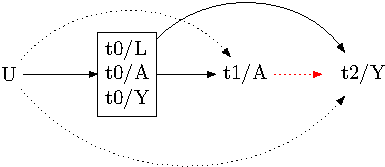
\includegraphics[width=0.8\textwidth,height=\textheight]{causal-dags_files/figure-pdf/fig-dag-6-1.pdf}

}

\caption{\label{fig-dag-6}Causal graph: adapted from Vanderweele et al's
three-wave panel design. The blue-dotted line indicates a reduction in
bias arising from the strategy of including baseline measures for the
exposure and outcome. For an unmeasured confounder U to bias the
exposure outcome association it would need to do so independently of
these baseline measures of the outcome and exposure. The graph
furthermore clarifies that by measuring confounders before the exposure
and the exposure before the outcome, we reduce the potential for reverse
causation, collider stratification, and mediator biases.}

\end{figure}

\hypertarget{step-4.-identify-observable-common-causes-of-the-exposure-and-the-outcome-and-group-them-under-simplified-labels}{%
\subsection{Step 4. Identify observable common causes of the exposure
and the outcome, and group them under simplified
labels}\label{step-4.-identify-observable-common-causes-of-the-exposure-and-the-outcome-and-group-them-under-simplified-labels}}

Next, we should identify all the potential confounders that, when
adjusted for, can eliminate any non-causal association between the
exposure and outcome. We should group these confounders under labels
where possible. In a three-wave panel design, these confounders are
typically recorded during the baseline wave, preceding the exposure. As
illustrated in Figure~\ref{fig-dag-mediator-solution}, recording
confounders before exposure minimises the potential for mediation bias.

\hypertarget{step-5.-gather-data-for-proxy-variables-of-unmeasured-common-causes-at-the-baseline-wave}{%
\subsection{Step 5. Gather data for proxy variables of unmeasured common
causes at the baseline
wave}\label{step-5.-gather-data-for-proxy-variables-of-unmeasured-common-causes-at-the-baseline-wave}}

If there exist any unmeasured factors influencing both the exposure and
outcome, but we lack direct measurements for them, efforts should be
made to include proxies for these factors, as outlined in
Figure~\ref{fig-dag-descendent-solution-2}. Again, even if this strategy
cannot be ensured to elimitate bias, it may reduce bias from unmeasured
confounding.

\hypertarget{step-6.-state-the-target-population-for-whom-the-causal-question-applies}{%
\subsection{Step 6. State the target population for whom the causal
question
applies}\label{step-6.-state-the-target-population-for-whom-the-causal-question-applies}}

We need to define for whom our causal inference applies. For this
purpose, it is useful to distinguish the concepts of source population
and target population, and between the concepts of generalisability and
transportability.

\begin{enumerate}
\def\labelenumi{\arabic{enumi}.}
\item
  \textbf{The source population} is the population from whom our sample
  is drawn.
\item
  \textbf{The target population} is the larger group for which we aim to
  apply our study's results. The closer the source matches the target in
  ways that are relevant to our causal questions, the stronger our
  causal inferences about the target population will be.
\item
  \textbf{Generalisability} refers to the ability to apply the causal
  effects estimated from a sample to the source population. Researchers
  in the human sciences know this concept as ``external validity.''
  Where:
\end{enumerate}

\begin{enumerate}
\def\labelenumi{\alph{enumi}.}
\tightlist
\item
  \(PATE\) denotes the population average treatment effect for the
  target population.
\item
  \(ATE_{\text{source}}\) denotes the average treatment effect in the
  source population.
\item
  \(W\) denotes a set of variables upon which the source and target
  population might differ when the research interest is in transporting
  resultes to a population other than that from which the source
  population is drawn.
\item
  \(T\) denotes a set of variables upon which the source and the target
  population might differ when the interest is in generalising beyond
  the population from which the source population is drawn.
\end{enumerate}

We may define \emph{generalisability} as:

\[PATE =  f(ATE_{\text{source}}, W)\]

Results generalise if the population average treatment effect in the
target population can be expressed as a function of the average
treatment effect in the source population and the set of variables,
\(W\), which differentiate the two populations. This function is a
mapping of the average treatment effect from the source population,
adjusted for the observed differences between the populations,
represented by \(W\). Here, \(f\) could be a model or a set of
transformations capturing the relationship between the source and target
populations' treatment effects, conditioned on \(W\). It might involve
rescaling, weighting, or modelling interactions.

\begin{enumerate}
\def\labelenumi{\arabic{enumi}.}
\setcounter{enumi}{3}
\tightlist
\item
  \textbf{Transportability} refers to the ability to extrapolate causal
  effects learned from a source population to a target population. It
  pertains to the transfer of causal knowledge across different settings
  or populations such that
\end{enumerate}

\[ATE_{\text{target}} \approx f(ATE_{\text{source}}, T)\]

This function similarly maps the average treatment effect from the
source population to a target population. However, the target population
in this case differs from the population from which the source was
drawn. The structures that enable inference are denoted by \(T\). The
function over \(T\) might be more complex, as it must handle potential
heterogeneity of effects and unobserved sources of bias. To assess
transportability we generally requier information about both the source
and target populations and an understanding of how the relationships
between treatment, outcome, and covariates might differ between the two
populations. Assessing transportability typically requires additional
data or specialist knowledge. In Section 4, we consider the concepts of
generalisability and transportability as they relate to sample
selection.

\hypertarget{step-7.-retention-is-critical}{%
\subsection{Step 7. Retention is
critical}\label{step-7.-retention-is-critical}}

For reasons we clarify in Part 4, retention of the original sample is
vital. Panel attrition not increases uncertainty by reducing the
effective sample size of a study at baseline, it opens novel pathways
for bias. Researchers must develop protocols for tracking individuals
over time as they change address, email, phone numbers, and names.
Moreover, developing and implementing strategies for motivating
retention of across the entire population of interest (not merely those
willing to volunteer for science) is critical for effective causal human
science. These strategies must be developed with specialist knowledge of
the population under study, and with the participation of people being
studied -- a topic for another article.

\hypertarget{summmary-part-3.}{%
\subsection{Summmary Part 3.}\label{summmary-part-3.}}

The general strategy for confounding control by three-wave panel designs
may be summarised in Figure~\ref{fig-dag-6}. The graph is adapted from
Tyler J. VanderWeele, Mathur, and Chen
(\protect\hyperlink{ref-vanderweele2020}{2020}) three-wave panel design.
The blue-dotted line indicates the possibility for unmeasured
confounding even after diminishing bias by including baseline measures
for the exposure and outcome. The causal diagram shows that for an
unmeasured confounder \(U\) to bias the exposure \(A_{t1}\to Y_{t2}\)
association it would need to do so independently of these baseline
measures of the exposure \(A_{t0}\) and exposure \(Y_{t0}\).
Figure~\ref{fig-dag-6} furthermore shows how panel researchers may
address reverse causation by controlling for both the exposure and
outcome at baseline. Figure~\ref{fig-dag-6} also reveals obtain an
estimate for the incidence of the effect rather than its prevelance.
Finally Figure~\ref{fig-dag-6} graph shows that by measuring confounders
before the exposure and the exposure before the outcome, we reduce the
potential for collider stratification and mediator bias, which, as we
saw in Part 2 arises when we unwittingly condition on a post-treatment
variable. Overall we discover that it is not enough to draw causal
diagrams. Causal diagrams reveal the mission-critical need for
collecting repeated measures data with particular attributes.

\hypertarget{part-4.-selection-bias-in-the-three-wave-panel-design}{%
\section{Part 4. Selection bias in the three wave panel
design}\label{part-4.-selection-bias-in-the-three-wave-panel-design}}

\hypertarget{selection-bias-at-the-start-of-study}{%
\subsection{Selection bias at the start of
study}\label{selection-bias-at-the-start-of-study}}

Selection bias may be defined generally the bias that arises when the
parameter of interest in a target population differs from the parameter
of interest in the subset of the population available for analysis --
that is from the source population
(\protect\hyperlink{ref-hernuxe1n2017}{M. A. Hernán 2017}). The source
population may differ from the target population in descriptive
parameters. In causal inference we are typically interested in how
selection bias may affect causal effect measures -- that is, in how such
difference affect causal contrasts on the some scale of interest
(difference, risk ratio, etc.) Here, we shall consider how causal
diagrams greatly facilitate progress in understanding such threats.
Before examining how, consider the following topology of confounding
developed by Suzuki and
colleagues(\protect\hyperlink{ref-suzuki2016}{Suzuki et al. 2016};
\protect\hyperlink{ref-suzuki2014}{Suzuki and Yamamoto 2014};
\protect\hyperlink{ref-suzuki2020}{Suzuki, Shinozaki, and Yamamoto
2020}), building on work by Tyler VanderWeele
(\protect\hyperlink{ref-vanderweele2012}{Tyler J. VanderWeele 2012}):

\begin{enumerate}
\def\labelenumi{\arabic{enumi}.}
\item
  \textbf{Confounding in distribution}: we say there is no confounding
  in distribution of the effect of the exposure on an outcome if the
  group that received each level of the exposure is representative of
  the target population.
\item
  \textbf{Confounding in expectation}: we say there is no confounding in
  expectation of the effect of the exposure on an outcome if the
  exposure assignment mechanism results in balance of confounders across
  each level of the exposure to be contrasted.
\item
  \textbf{Confounding in measure}: there is no confounding in measure of
  the effect of the exposure on an outcome if a particular measure of
  interest is equivalent to the corresponding causal measure in the
  target population. This concept is important because, as we noted in
  our discussion of interaction, whether we infer a causal effect may
  depend on the scale of the causal effect measure. An effect may be
  present on the difference scale but not present on the relative-risk
  scale, and vice versa. If selection introduces an effect modifier, the
  scale at which an effect is measured may affect whether an how results
  generalise (or transport) from the source to target population.
\item
  \textbf{Realised confounding}: we say there is no realised confounding
  of the effect of the exposure on an outcome if a particular exposure
  assignment results in balance, irrespective of the exposure assignment
  mechanism. This concept is important because even in randomised
  experiments, randomisation may fail to remove chance imbalances in the
  distributions of confounders in the exposures. We may have no
  confounding in expectation yet the experimental effect estimate might
  differ for the source and target populations.
\end{enumerate}

Eaach of these four concepts is variously used in discussions of
``confounding.'' All are important when evaluating the scientific
contribution of a study. Yet each concept brings different issues into
focus.

With these distinction to hand, consider
Figure~\ref{fig-selection-under-the-null}, which presents a scenario in
which there is no (marginal) causal effect of the exposure on the
outcome, yet there is selection into the study. We imagine randomisation
such that there is no path from any other node into \(A\). Let us assume
randomisation succeeded. Finally, we imagine there there is no causal
path from \(A \to Y\). As evident in
Figure~\ref{fig-selection-under-the-null} there is no confounding in the
expectation, nor is there confounding in distribution. The null effect
estimate returned from the study will honour the true null effect in the
population. We might say that selection does lead to ``confounding in
distribution for confounding in expectation.'' Or more simply, despite
selection, the null effect in the source population is unbiased for the
target population. Our null results generalise (see:
(\protect\hyperlink{ref-hernuxe1n2004b}{Miguel A. Hernán,
Hernández-Díaz, and Robins 2004}), see also
(\protect\hyperlink{ref-greenlands.1977a}{Greenland, S. 1977})).

\begin{figure}

{\centering 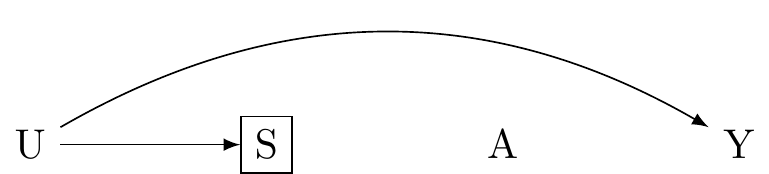
\includegraphics[width=0.6\textwidth,height=\textheight]{causal-dags_files/figure-pdf/fig-selection-under-the-null-1.pdf}

}

\caption{\label{fig-selection-under-the-null}Selection under the null.
An unmeasured variable affects selection into the study and the outcome.
D-separation is preserved there is no confounding in expectation.}

\end{figure}

Figure~\ref{fig-selection-off-the-null} presents a different scenario in
which there selection bias for the population parameter: the association
in the population of selected individuals differs from the causal
association in the target population. Hernán calls this ``selection bias
off the null'' (\protect\hyperlink{ref-hernuxe1n2017}{M. A. Hernán
2017}) and Lu et al call this ``type 2 selection bias''
(\protect\hyperlink{ref-lu2022a}{Lu et al. 2022}) This bias occurs
because the selection into the study occurs on an effect modifier for
the effect of the exposure on the outcome. In this scenario there is
what Suzuki et al call ``confounding in distribution for the confounding
in expectation.'' That is, although the causal effect of \(A\to Y\) is
unbiased for the exposed and unexposed in the source population, the
effect estimate does not generalise to the exposed and unexposed in the
target population: \(PATE \cancel{\approx} ATE_{\text{sample}}\).

\begin{figure}

{\centering 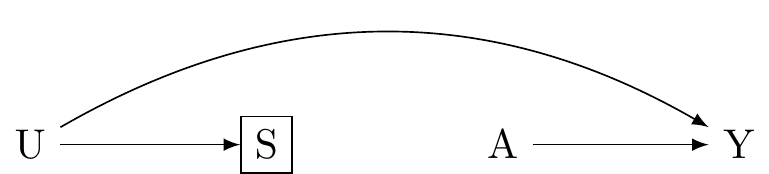
\includegraphics[width=0.6\textwidth,height=\textheight]{causal-dags_files/figure-pdf/fig-selection-off-the-null-1.pdf}

}

\caption{\label{fig-selection-off-the-null}Selection off the null: an
unmeasured variable affects selection into the study and the outcome.
Here the exposure affects the outcome. Although D-separation is
preserved, there there is confounding in distribution.}

\end{figure}

There has been considerable work investigating the conditions under
which causal estimates for a target population may be identified when
the source population differs from the target population
(\protect\hyperlink{ref-lu2022a}{Lu et al. 2022}), i.e.~whether we may
obtain a function such that \(PATE = f(ATE_{\text{source}}, W)\).
Whether results transport to populations that systematically differ from
the source population -- i.e.~whether we may obtain a function such that
\(ATE_{\text{target}} \approx f(ATE_{\text{source}}, T)\) -- is also an
area of active research
(\protect\hyperlink{ref-bareinboim2022a}{Bareinboim, Tian, and Pearl
2022}; \protect\hyperlink{ref-deffner2022a}{Deffner, Rohrer, and
McElreath 2022}). As @Lu et al. (\protect\hyperlink{ref-lu2022a}{2022})
point out, type 2 selection bias should be addressed during the design
and analytic stage by accurately measuring and properly adjust for a
sufficient set of covariates that affect selection \(\framebox{S}\) and
the outcome in the target population. Moreover, as Suzuki, Shinozaki,
and Yamamoto (\protect\hyperlink{ref-suzuki2020}{2020}) suggest, when
drawing a causal diagramme, it is vital to present confounding as it
exists in the target population (see especially their examples in the
appendix.)

In panel designs there is additionally a constant threat of selection
occurring \emph{after} enrolment into the study. We next put
chronological causal diagrams to use in making sense of this threat, and
to derive practical advice.

\hypertarget{selection-bias-in-which-both-the-exposure-and-outcome-affect-selection}{%
\subsection{Selection bias in which both the exposure and outcome affect
selection}\label{selection-bias-in-which-both-the-exposure-and-outcome-affect-selection}}

We next use causal diagrams to clarify biases arising from panel
attrition. Panel attrition can be viewed as a special case of selection
bias because the participants who continue in a longitudinal study may
differ from those who drop out in ways that generate structural biases.

Figure~\ref{fig-dag-8-5}, describes a scenario in one in which both the
exposure and the true outcome affect panel attrition, biasing the
observed association between the exposure and the measured outcome in
the remaining sample. Here we present the problem as an instance of
collider stratification bias. The problem can be equivalently viewed as
one of directed measurement error, described in the next section in
Figure~\ref{fig-dag-indep-d-effect}. Either way, restricting analysis to
the retained sample introduces bias in the the causal effect estimate by
opening a backdoor path from the exposure to the outcome.

\begin{figure}

{\centering 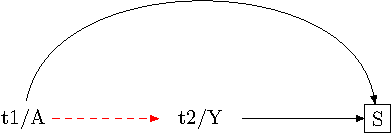
\includegraphics[width=0.8\textwidth,height=\textheight]{causal-dags_files/figure-pdf/fig-dag-8-5-1.pdf}

}

\caption{\label{fig-dag-8-5}Causal graph:outcome and exposure affect
attrition.}

\end{figure}

\hypertarget{selection-bias-in-a-three-wave-panel}{%
\subsection{Selection bias in a three-wave
panel}\label{selection-bias-in-a-three-wave-panel}}

Figure Figure~\ref{fig-dag-8} shows selection bias manifest in a
three-wave panel design when loss-to-follow-up results in a systematic
disparity between the baseline and follow-up source populations. The red
dashed lines in the diagram represent an open back-door path,
symbolising a potential indirect association between the exposure and
the outcome. Upon considering only the selected sample (i.e., when we
condition on the selected sample \(\framebox{S}\)), we may create or
obscure associations that would not be evident in the original source
population at baseline.

\begin{figure}

{\centering 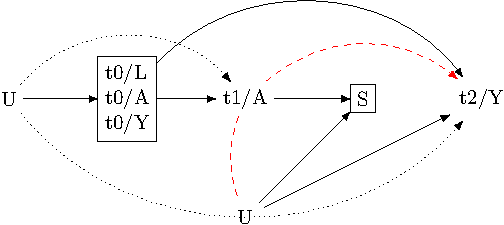
\includegraphics[width=0.8\textwidth,height=\textheight]{causal-dags_files/figure-pdf/fig-dag-8-1.pdf}

}

\caption{\label{fig-dag-8}Causal graph: three-wave panel design with
selection bias. The red dashed paths reveal the open backdoor path
induced by conditioning on the selected sample.}

\end{figure}

\hypertarget{unmeasured-confounder-affects-outcome-and-variable-that-affects-attrition}{%
\subsection{Unmeasured confounder affects outcome and variable that
affects
attrition}\label{unmeasured-confounder-affects-outcome-and-variable-that-affects-attrition}}

Figure Figure~\ref{fig-dag-8-2} presents another problem of selection
bias in a three-wave panel design. This diagram shows how an unmeasured
confounder, U\(_S\), can simultaneously influence the outcome variable
Y\(_{t2}\) and another variable, L\(_{t2}\), responsible for attrition
(i.e., the drop-out rate, denoted as \(\framebox{S}\)). In this
instance, the exposure variable, \(A_{t1}\), can impact L\(_{t2}\),
which subsequently affects attrition, \(\framebox{S}\). If the study's
selected sample descends from L\(_2\), the selection effectively
conditions on L\(_{t2}\), introducing potential bias into the analysis.
The diagram marks this possible biasing pathway with red-dashed lines.
Ordering the nodes chronologically elucidates the temporal sequence of
these events, allowing for a clearer assessment of potential bias
sources relevant to a three-wave panel design.

\begin{figure}

{\centering 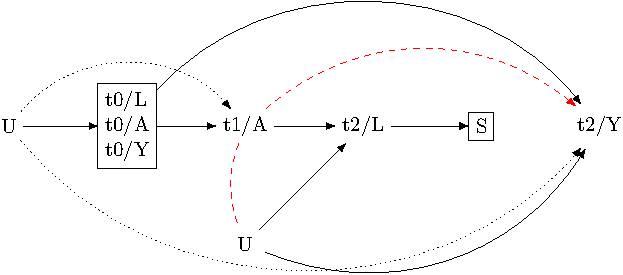
\includegraphics[width=0.8\textwidth,height=\textheight]{causal-dags_files/figure-pdf/fig-dag-8-2-1.pdf}

}

\caption{\label{fig-dag-8-2}Causal graph: three-wave panel design with
selection bias: example 2: Unmeasured confounder U\_S, is a cause of
both of the outcome Y\_2 and of a variable, L\_2 that affects attrition,
S. The exposure A affect this cause L\_2 of attrition, S. The selected
sample is a descendent of L\_2. Hence selection is a form of
conditioning on L\_2. Such conditioning opens a biasing path, indicated
by the red-dashed lines.}

\end{figure}

\hypertarget{summary-part-4}{%
\subsection{Summary Part 4}\label{summary-part-4}}

In this section, we have used causal diagrams to clarify sources of
confounding arising from selection bias in the setting of longitudinal
research, revealing further scope for the practical applications of
causal diagrams when planning research. The key advice is as follows.

\begin{enumerate}
\def\labelenumi{\arabic{enumi}.}
\item
  To ensure generalisability, wherever possible, sample broadly from the
  target population. Ensure that all effect-modifiers are measured. To
  better assess the role that effect-modification may play, draw your
  causal diagramme for the target population.
\item
  Ensure the strongest possible retention of your sample. Ideally we
  would retain all participants. However, perfect retention is almost
  always impractical. When estimating causal effects, researchers must
  instead employ methods such as multiple-imputation or inverse
  probability of censoring weights to restore balance. These are not
  fail-safe methods. I reiterate the need for sensitivity analyses.
\end{enumerate}

\hypertarget{part-5.-measurement-and-confounding-in-the-three-wave-panel-design}{%
\section{Part 5. Measurement and confounding in the three wave panel
design}\label{part-5.-measurement-and-confounding-in-the-three-wave-panel-design}}

Here we causal diagrams to clarify bias from measurement error,
revealing implications for research design. Following Miguel A. Hernán
and Cole (\protect\hyperlink{ref-hernuxe1n2009}{2009}), we first define
structural concepts of measurement error and draw causal diagrams to
understand how they may bias causal effect estimates (see also
(\protect\hyperlink{ref-vanderweele2012a}{Tyler J. VanderWeele and
Hernán 2012})).

\hypertarget{uncorrelated-non-differential-undirected-measurement-error}{%
\subsubsection{\texorpdfstring{1. \textbf{Uncorrelated non-differential
(undirected) measurement
error}}{1. Uncorrelated non-differential (undirected) measurement error}}\label{uncorrelated-non-differential-undirected-measurement-error}}

As shown in Figure~\ref{fig-dag-uu-null}, uncorrelated non-differential
measurement error occurs when the errors in measurement of the exposure
and outcome are not related.

To clarify,consider again the task of estimating the causal effect of
beliefs in big Gods on social complexity. Suppose ancient societies
randomly omitted or recorded details about both beliefs in Big Gods and
indicators of social complexity in their records. Or equivalently,
suppose that such records were not preserved equally across cultures for
reasons unrelated to these parameters. In this case, errors in the
documentation of both variables would be random. That is, the errors
would not be related to the intensity of the beliefs in Big Gods or the
level of social complexity. This example provides an instance of
uncorrelated and non-differential error, and is presented in
Figure~\ref{fig-dag-uu-null}.

Uncorrelated non-differential measurement error does not create bias
under the null. As evident from Figure~\ref{fig-dag-uu-null},
d-separation is preserved. Our equivalently, there are no open back
doors on the graph. However, when there is a true effect of the exposure
on the outcome, non-differential measurement error generally leads to an
attenuation of the true effect estimate. For this reason, uncorrelated
non-differential measurement error can be problematic for inference even
though it does not induce structural bias under the null.

\begin{figure}

{\centering 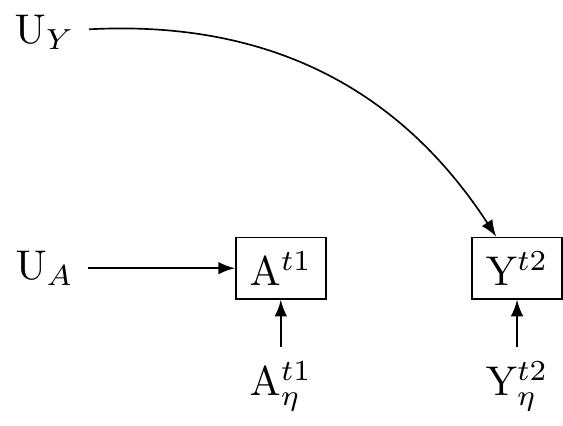
\includegraphics[width=0.6\textwidth,height=\textheight]{causal-dags_files/figure-pdf/fig-dag-uu-null-1.pdf}

}

\caption{\label{fig-dag-uu-null}Uncorrelated non-differential
measurement error does not bias estimates under the null, however may
attenuate true effects.}

\end{figure}

\hypertarget{uncorrelated-differential-directed-measurement-error}{%
\subsubsection{\texorpdfstring{2. \textbf{Uncorrelated differential
(directed) measurement
error}}{2. Uncorrelated differential (directed) measurement error}}\label{uncorrelated-differential-directed-measurement-error}}

As shown in Figure~\ref{fig-dag-indep-d-effect}, uncorrelated
differential (or directed) measurement error occurs when the errors in
measurement are related to the level of exposure or outcome, but not to
each other. For instance, societies with stronger `beliefs in Big Gods'
might cause a society to provide more or less detailed records of
`social complexity'. However, in the absence of any intervention on
beliefs in Gods, there is no association between the measurement errors.
Here, the errors are differential as they depend on the intensity of
religious beliefs, but uncorrelated as the errors in documenting
`beliefs in Big Gods' and `social complexity' are otherwise independent
of each other. Uncorrelated differential (or directed) measurement error
is presented in Figure~\ref{fig-dag-indep-d-effect} and leads to bias
under the null, indicated by the red path. Or equivalently, uncorrelated
differential (or directed) measurement error opens a back-door path
between the exposure and the outcome.

Note that the bias presented in Figure~\ref{fig-dag-indep-d-effect},
which is an example of directed measurement error, also describes the
bias we considered when there is panel attrition, and which the exposure
and affects selection (see: Figure~\ref{fig-dag-8-5}). In that scenario,
the outcome in the selected group is measured with error -- it no long
represents the measurement of the outcome in the source population at
baseline -- and further more, this error is affected by the exposure.
The previous example described bias in estimation from the vantage point
of collider stratification, however the example may be equally explained
from the more general vantage point of directed measurement bias.

\begin{figure}

{\centering 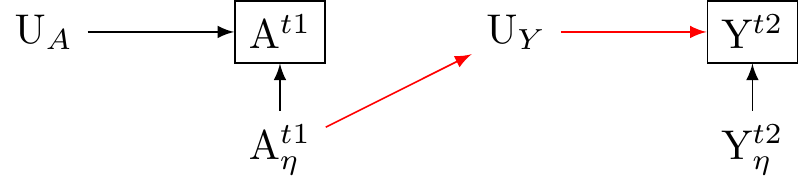
\includegraphics[width=1\textwidth,height=\textheight]{causal-dags_files/figure-pdf/fig-dag-indep-d-effect-1.pdf}

}

\caption{\label{fig-dag-indep-d-effect}Directed independent
(uncorrelated) measurement error biases effect estimates, indicated by
the red path. The selection bias presented in the previous graph is an
instance of directed independent measurement error.}

\end{figure}

\hypertarget{correlated-non-differential-undirected-measurement-error}{%
\subsubsection{\texorpdfstring{3. \textbf{Correlated non-differential
(undirected) measurement
error}}{3. Correlated non-differential (undirected) measurement error}}\label{correlated-non-differential-undirected-measurement-error}}

As shown Figure~\ref{fig-dag-dep-u-effect} correlated non-differential
(undirected) measurement error occurs when the errors in measuring both
the exposure and outcome are related to each other, but not to the level
of exposure or outcome. The scenario is presented in
Figure~\ref{fig-dag-dep-u-effect}. Imagine that some societies had more
advanced record-keeping systems that resulted in more accurate and
detailed accounts of both `beliefs in Big Gods' and `social complexity'
and furthermore that the record keepers provide better information about
religious beliefs. These errors between beliefs in big Gods and social
complexity might be correlated because the accuracy of records on both
variables is influenced by the same underlying factor (the
record-keeping abilities), but they are non-differential insofar as true
religious beliefs and true social complexity do not affect bias in the
record keeping. Correlated non-differential measurement error may induce
bias under the null, indicated by the red path in
Figure~\ref{fig-dag-dep-u-effect}.

\begin{figure}

{\centering 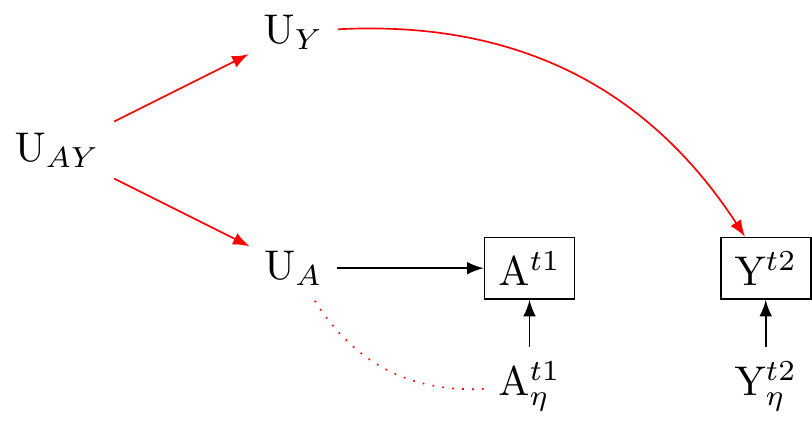
\includegraphics[width=0.8\textwidth,height=\textheight]{causal-dags_files/figure-pdf/fig-dag-dep-u-effect-1.pdf}

}

\caption{\label{fig-dag-dep-u-effect}Correlated undirected measurement
error can dilute the estimates of true effects, indicated by the red
path.}

\end{figure}

\hypertarget{correlated-differential-directed-measurement-error}{%
\subsubsection{\texorpdfstring{4. \textbf{Correlated differential
(directed) measurement
error}}{4. Correlated differential (directed) measurement error}}\label{correlated-differential-directed-measurement-error}}

As presented in Figure~\ref{fig-dag-d-d}, correlated differential
(directed) measurement error occurs when the errors in measurement are
related to each other and also to the level of exposure or outcome.
Suppose that societies with stronger beliefs in big Gods tend to record
their both their religious beliefs and social structure in more detail
and that this work conducted by religious elites. In this case, the
errors may be both correlated and differential if societies with beliefs
in big Gods tend to favour the religious elites who keep biased records.

\begin{figure}

{\centering 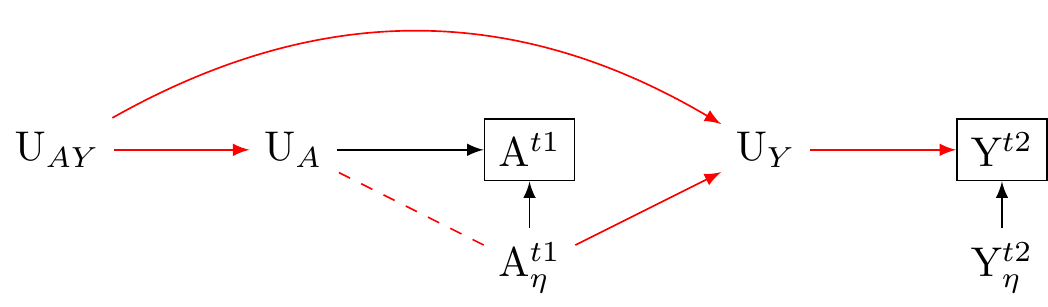
\includegraphics[width=1\textwidth,height=\textheight]{causal-dags_files/figure-pdf/fig-dag-d-d-1.pdf}

}

\caption{\label{fig-dag-d-d}Directed dependent (correlated) measurement
error biases effect estimates. Here, the exposure affects the
measurement error of the outcome. Additionally, the measurement errors
of the exposure and outcome are correlated. These dynamics open pathways
for bias.}

\end{figure}

\hypertarget{comparative-research-viewed-as-correlated-undirected-measurment-error}{%
\subsection{Comparative research viewed as correlated undirected
measurment
error}\label{comparative-research-viewed-as-correlated-undirected-measurment-error}}

Against invariance testing, we should approach comparative research from
the vantage point of correlated measurement error. Amending
Figure~\ref{fig-dag-dep-u-effect}. Selecting on unmeasured correlated
error structures in the world we have
Figure~\ref{fig-dag-dep-u-effect-selection}.

Were we to select from a setting in which there was no systematic
(correlated) error structures between the measurements of the exposures
and the measurements of the outcomes we would avoid such confounding.

Note that it is not merely a matter of transporting results from the
sample population to another population. Rather, the act of selection
induces bias.

\begin{figure}

{\centering \includegraphics[width=1\textwidth,height=\textheight]{causal-dags_files/figure-pdf/fig-dag-dep-u-effect-selection-1.pdf}

}

\caption{\label{fig-dag-dep-u-effect-selection}Measurement bias in
comparative cross-cultural research}

\end{figure}

\hypertarget{how-controlling-for-baseline-measures-mitigates-against-correlated-measurement-errors}{%
\section{How controlling for baseline measures mitigates against
correlated measurement
errors}\label{how-controlling-for-baseline-measures-mitigates-against-correlated-measurement-errors}}

Controlling for a baseline measure of the exposure and the outcome is
essentially controlling for potential confounding caused by any
time-invariant characteristics that might influence both the exposure
and the outcome. Such confounding is suppressed because any effect of
these characteristics on the outcome is supposed to be the same at
baseline and at follow-up, assuming no interaction with time.

When it comes to measurement error, the situation is somewhat different.
If the exposure and outcome are both measured with error, and the errors
are correlated, this would typically introduce bias in our estimate of
the causal effect. We have seen that if this this error is systematic
and non-differential, it may lead to an attenuation of the estimated
causal effect.

Including baseline measurements of the exposure and outcome in our model
can, in theory, help mitigate this bias. This is because the model
would, in effect, be using the change in the exposure and outcome from
baseline to follow-up to estimate the causal effect. If the measurement
error is consistent across time (i.e., it is a constant amount or a
constant proportion of the true value), then using these change scores
could help to control for it.

However, this assumes that the measurement error has no directionality
and is not differential with respect to time. If the measurement error
varies over time or in relation to other variables in the model, then
controlling for baseline measurements may not fully correct for it.

Here is a simple mathematical representation of the conditions. Let
\(A_0\), \(A_1\) denote the exposure at baseline and follow-up, and let
\(Y_0\), \(Y_1\) denote the outcome at baseline and follow-up. The true
values are denoted without primes, and the measured values with primes.
We assume the measurement error is additive:

\(A'_0 = A_0 + U_0\),

\(A'_1 = A_1 + A_1\),

\(Y'_0 = Y_0 + V_0\),

\(Y'_2 = Y_2 + V_2\),

where \(U_0\), \(U_1\) are the measurement errors for the exposure at
baseline and follow-up, and \(V_0\), \(V_2\) are the measurement errors
for the outcome at baseline and follow-up. If the errors are correlated,
then \(Cov(U_0, V_0) \neq 0\) and/or \(Cov(U_1, V_2) \neq 0\).

In a model that includes \(A'_0\) and \(Y'_0\) as covariates, the
estimated effect of \(A'_1\) on \(Y'_2\) is essentially the estimated
effect of the change in the exposure from baseline to follow-up on the
change in the outcome from baseline to follow-up, controlling for the
baseline measures. This will mitigate the bias arising from to
correlated errors if the following conditions hold:

\(E(U_0) = E(U_1)\) and \(E(V_0) = E(V_2)\) (i.e., the expectation of
the measurement errors does not change over time),

\(Cov(U_0, V_2) = Cov(U_1, V_2)\) (i.e., the correlation between the
errors does not change over time).

If these conditions do not hold, then the bias may not be fully
controlled for, and other methods may be needed.\footnote{I have assumed
  that the measurement errors are additive and undirected. If the errors
  are multiplicative or have some other form, or if they vary with the
  level of the true values or with other variables in the model, then
  this simple analysis might not apply.}

\hypertarget{casual-diagrams-clarify-the-structural-assumptions-underlying-classical-measurement-theory}{%
\subsection{Casual diagrams clarify the structural assumptions
underlying classical measurement
theory}\label{casual-diagrams-clarify-the-structural-assumptions-underlying-classical-measurement-theory}}

Researchers working in cultural evolution often incorporate multi-item
constructs into their panel study designs, a practice which is aligned
with the recommendations of conventional psychometric theory. However,
classical psychometric theory emerged without the benefit of causal
theories. As noted by Tyler VanderWeele, issues arise when evaluating
the causal assumptions of formative and reflective models
(\protect\hyperlink{ref-vanderweele2022}{Tyler J. VanderWeele 2022a}).
Let us first consider the issues before expanding on how they manifest
in panel research.

There are two prevailing approaches in this area: formative and
reflective models. The focus here will be on reflective models, though
it should be noted that the issues identified also apply to formative
models, as outlined by VanderWeele {[}Tyler J. VanderWeele
(\protect\hyperlink{ref-vanderweele2022}{2022a}){]}\footnote{In a
  formative model, the observed variables are thought to cause the
  latent variable. As in the reflective model, there is a single latent
  variable. This latent variable, however, is considered the effect of
  the underlying indicators. In mathematical terms, if \(\eta\)
  represents the latent variable, \(\lambda_i\) denotes the weight for
  \(X_i\) (the observed variable), and \(\varepsilon\) is the error
  term, the latent variable \(\eta\) can be described as a composite of
  the observed variables \(X_i\), expressed as:
  \(\eta = \sum_i\lambda_i X_i\).}.

In a reflective model, researchers posit that a latent variable gives
rise to the observed indicators. Each observed variable (or indicator)
is seen as a `reflection' or manifestation of the latent variable. If
\(X_i\) is an observed variable (indicator), \(\lambda_i\) is the factor
loading for \(X_i\), \(\eta\) is the latent variable, and
\(\varepsilon_i\) is the error term associated with \(X_i\), the
reflective model can be formulated as:

\[X_i = \lambda_i \eta + \varepsilon_i\]

Factor analysis typically assumes a common latent variable, which is
responsible for the correlations observed among the indicators. The
causal assumptions linked to this concept are demonstrated in Figure
Figure~\ref{fig-dag-latent-1}.

\begin{figure}

{\centering 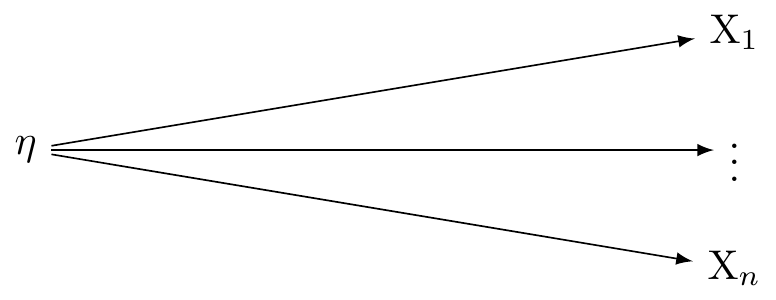
\includegraphics[width=0.6\textwidth,height=\textheight]{causal-dags_files/figure-pdf/fig-dag-latent-1-1.pdf}

}

\caption{\label{fig-dag-latent-1}Reflective model: assume univariate
latent variable η giving rise to indicators X1\ldots X3. Figure adapted
from VanderWeele: doi: 10.1097/EDE.0000000000001434}

\end{figure}

The statistical implications of the \textbf{reflective model} suggest
that the observed variables (indicators) are reflections or
manifestations of the latent variable, which is mathematically expressed
as \(X_i = \lambda_i \eta + \varepsilon_i\). The factor analytic
tradition goes one step further by proposing a structural assumption
that a univariate latent variable causally affects the observed
variables. Hence, the reflective model yields
\(X_i = \lambda_i \eta + \varepsilon_i\), which is assumed to underpin
the structural assumptions shown in Figure
Figure~\ref{fig-structural-assumptions-reflective-model}.

\begin{figure}

{\centering 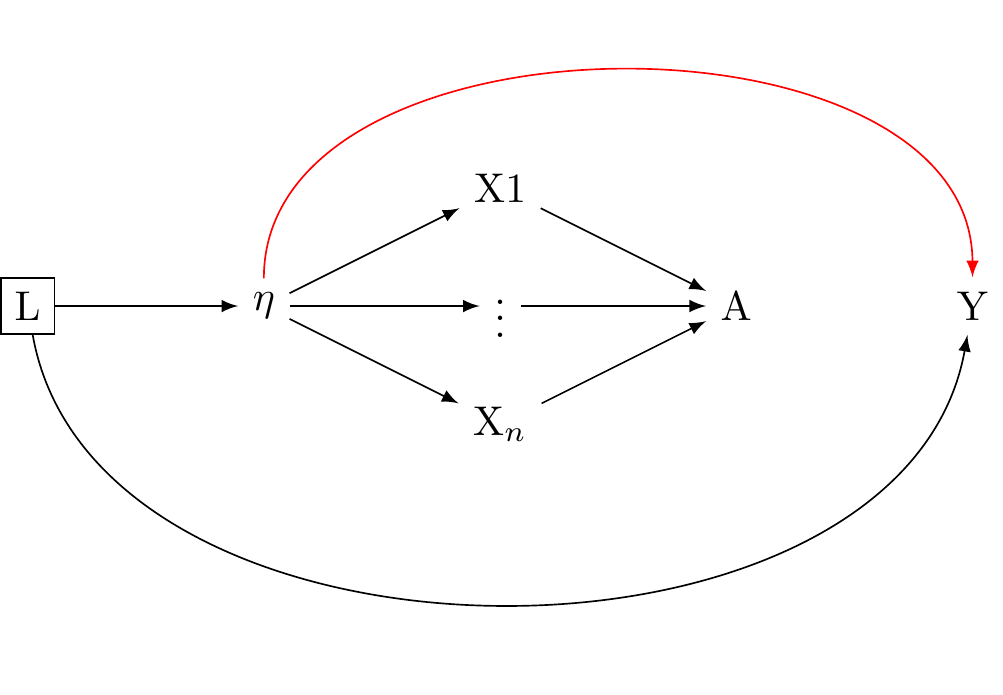
\includegraphics[width=0.8\textwidth,height=\textheight]{causal-dags_files/figure-pdf/fig-structural-assumptions-reflective-model-1.pdf}

}

\caption{\label{fig-structural-assumptions-reflective-model}Reflective
Model: causal assumptions. Figure adapted from VanderWeele: doi:
10.1097/EDE.0000000000001434}

\end{figure}

VanderWeele notices that while the statistical model
\(X_i = \lambda_i \eta + \varepsilon_i\) concurs with the structural
assumptions in Figure
Figure~\ref{fig-structural-assumptions-reflective-model}, it can also
align with various causal models. For instance, the statistical model is
compatible with the reality presented in @
fig\_dag\_multivariate\_reality\_again, where unique latent variables
give rise to distinct indicators, some of which (but not necessarily
all) have a causal effect on the outcome. The statistical model does not
provide clarity about which structural model is accurate. Additionally,
the assumption that a univariate underlying reality forms the basis of
the formative and reflective latent factor models, which is a much
stronger assumption than has been previously acknowledged in
psychometric literature. For widely used measures these assumptions fail
to withstand empirical scrutiny
(\protect\hyperlink{ref-vanderweele2022b}{Tyler J. VanderWeele and
Vansteelandt 2022}).

\begin{figure}

{\centering 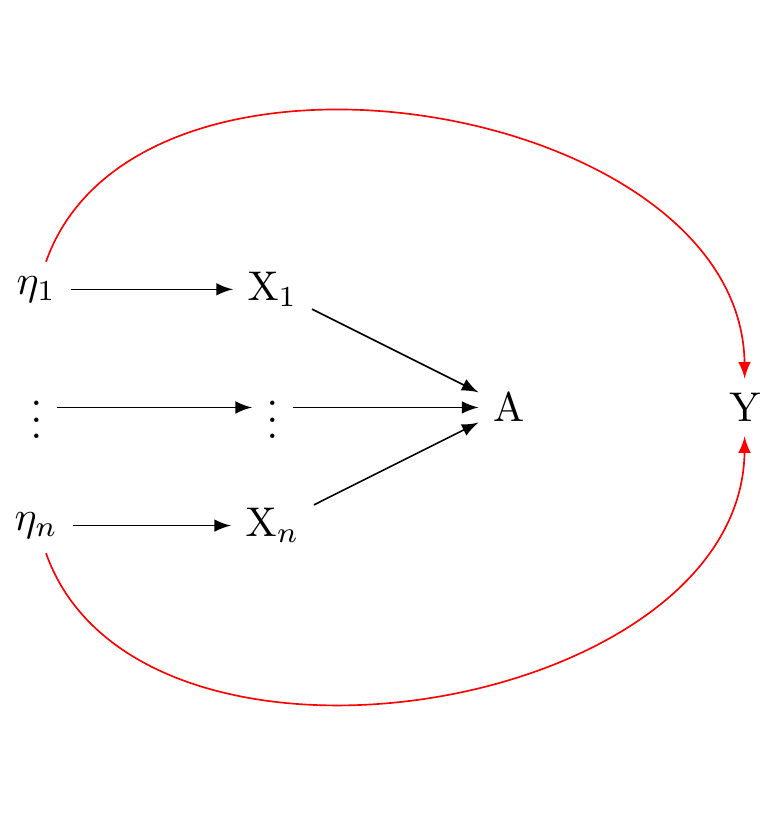
\includegraphics[width=0.6\textwidth,height=\textheight]{causal-dags_files/figure-pdf/fig_dag_multivariate_reality_again-1.pdf}

}

\caption{Multivariate reality gives rise to the indicators, from which
we draw our measures. Figure adapted from VanderWeele: doi:
10.1097/EDE.0000000000001434}

\end{figure}

VanderWeele suggests that construct measures can still be utilised in
applied research by extending the theory of causal inference under
multiple interventions to factor models
(\protect\hyperlink{ref-vanderweele2022a}{Tyler J. VanderWeele 2022b})
(for a detailed discussion, refer to Appendix 1).

By expressing our measured variables as functions of indicators, and
assuming the true underlying reality as a coarsened measure of a
potentially complex latent reality, we can consistently estimate causal
effects under this extended theory. This approach is illustrated in
Figure~\ref{fig-dag-multiple-version-treatment-applied-measurement}.

\begin{figure}

{\centering 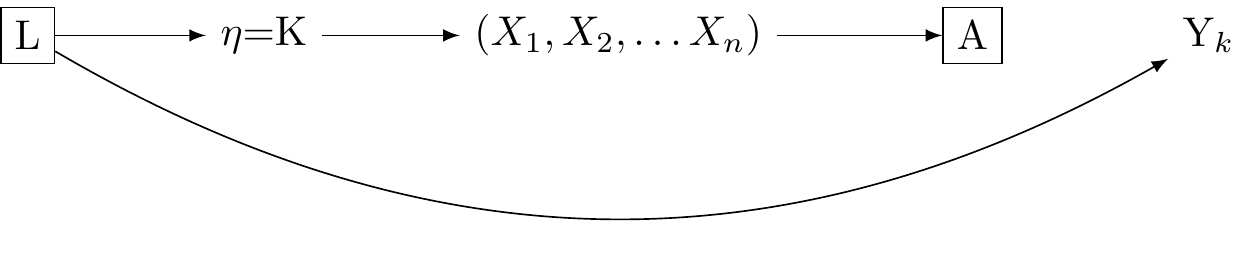
\includegraphics[width=0.8\textwidth,height=\textheight]{causal-dags_files/figure-pdf/fig-dag-multiple-version-treatment-applied-measurement-1.pdf}

}

\caption{\label{fig-dag-multiple-version-treatment-applied-measurement}Multiple
Versions of treatment applied to measuremen.Figure adapted from
VanderWeele: doi: 10.1097/EDE.0000000000001434}

\end{figure}

\hypertarget{measurement-error-and-construct-measures}{%
\subsection{Measurement Error and Construct
Measures}\label{measurement-error-and-construct-measures}}

Consider a three wave panel where, for simplicity, we assume no
unmeasured confounding is present. Our exposure \(A\) can be measured by
a function of indicators, denoted as \(A_{f(A_1, A_2, ..., A_n)}\),
forming a coarsened state from a multivariate reality. Each element of
this reality has a corresponding structural component, denoted as
\(\eta_{A_1}, \eta_{A_2}, ..., \eta_{A_n}\). These components are
measured with their respective error terms,
\(U\eta_{A_1}, U\eta_{A_2}, ..., U\eta_{A_n}\).

Similar to the exposure, our outcome Y can be conceptualised as a
function of indicators, \(Y_{f(Y_1, Y_2, ..., Y_n)}\), of a latent
reality. This reality is expressed through the latent components
\(\eta_{Y_1}, \eta_{Y_2}, ..., \eta_{Y_n}\), each having their
associated error term \(U\eta_{Y_1}, U\eta_{Y_2}, ..., U\eta_{Y_n}\).

Figure~\ref{fig-dag-coarsen-measurement-error} illustrates the assumed
reality. It shows possible paths for confounding via directed
measurement error. Each path is represented by a structural component
\(\eta_{A_n}\) and its associated error term \(U\eta_{Y_n}\). Here we
present three possible confounding paths that are possible from directed
measurement error.

Note that the potential for confounding arising from measurement error
in panel designs depends fundamentally on the particular relationships
and dependencies among variables, not merely their quantity. However, we
can see here that, theoretically, a larger number of latent states or
error terms could amplify the possibilities for confounding. In a
simplistic scenario, \emph{every} latent variable associated with an
exposure could affect each error term of an outcome, leading to an
expansive network of confounding paths.

This underscores thinking very carefully about the composite terms when
using psychological constructs. In many cases researchers might wish to
use single item measures. A general rule here is not possible. Every
case must be considered with careful attention to the meanings of the
items, their likely interpretations and their potential causal
underpinnings over time.

\begin{figure}

{\centering 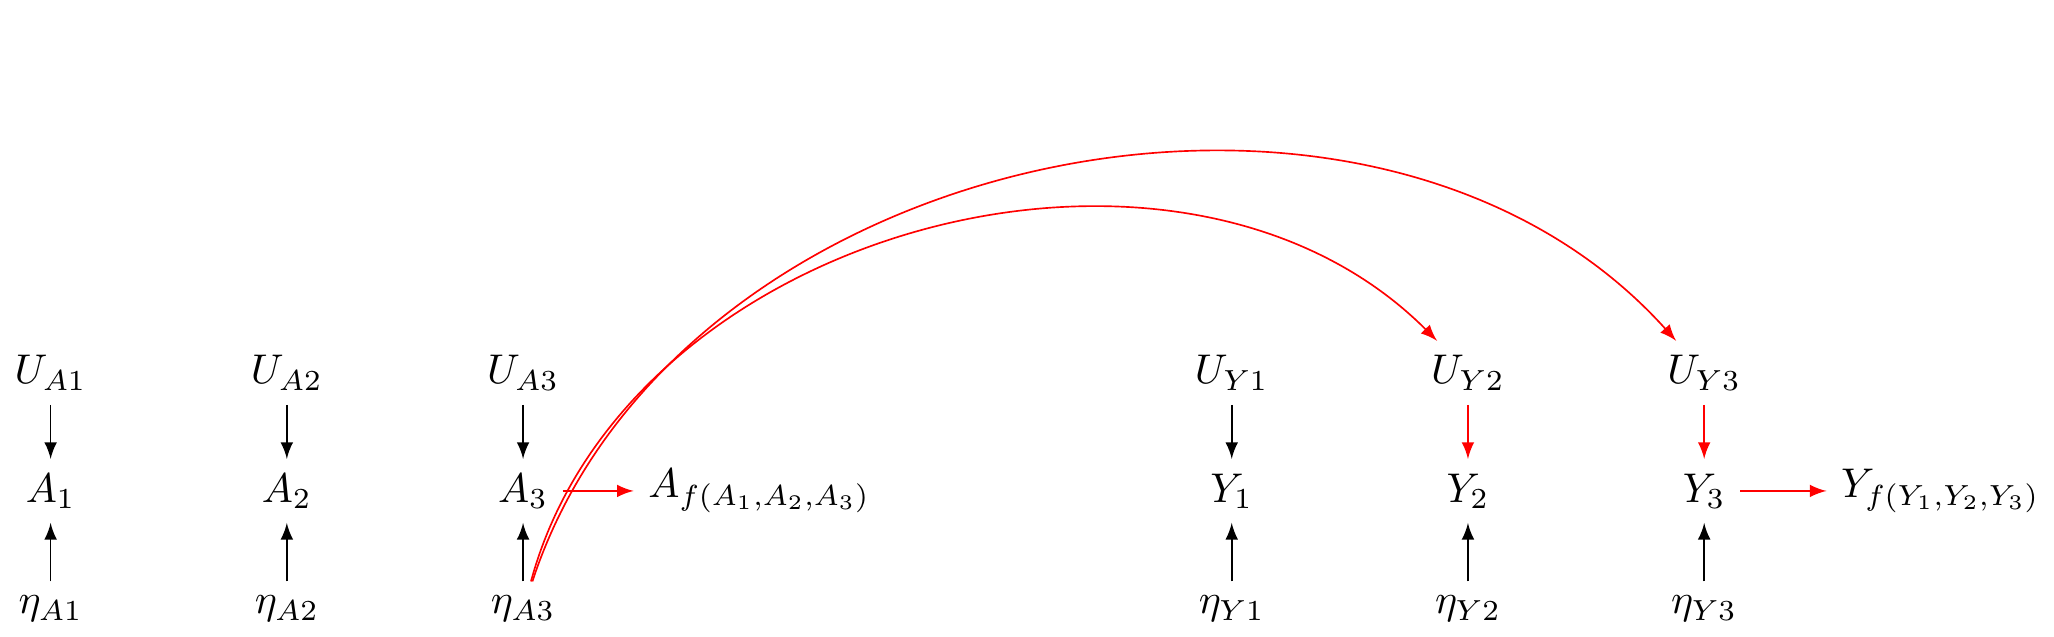
\includegraphics[width=1\textwidth,height=\textheight]{causal-dags_files/figure-pdf/fig-dag-coarsen-measurement-error-1.pdf}

}

\caption{\label{fig-dag-coarsen-measurement-error}Where there are many
indicators of a psychological construct, there are many opportunities
for additional confounding by directed measureemnt error.}

\end{figure}

\hypertarget{summary-part-5.}{%
\subsection{Summary Part 5.}\label{summary-part-5.}}

In Part 5, the focus is on understanding measurement and confounding
errors in the three-wave panel design using causal diagrams. We discuss
four types of measurement errors and how they may affect research
results. These include uncorrelated non-differential (undirected)
measurement error, uncorrelated differential (directed) measurement
error, correlated non-differential (undirected) measurement error, and
correlated differential (directed) measurement error.

Within a three-wave panel design, I discussed an example where the
estimation of the effect of self-reported religious service attendance
on self-reported monthly donations to charity might be influenced by
systematic errors.

I emphasised that while adjusting for baseline exposure can help reduce
confounding and isolate incidence effects, it is not a solution for all
biases. Attention must be given to the quality of measurements at all
time points and the design of the questions to avoid potential biases,
such as presentation bias. causal diagrams are helpful in clarifying
these complex structures confounding.

\hypertarget{conclusions}{%
\subsection{Conclusions}\label{conclusions}}

\hypertarget{summary-of-advice}{%
\subsection{Summary of advice}\label{summary-of-advice}}

\begin{enumerate}
\def\labelenumi{\arabic{enumi}.}
\item
  \textbf{Define all variables clearly}: Ensure that all variables in
  your causal graph are distinctly defined.
\item
  \textbf{Define novel conventions}: if you are using unique conventions
  in your diagram, such as coloured arrows to indicate induced
  confounding, make sure to define them.
\item
  \textbf{Embrace minimalism}: include only the nodes and edges that
  clarify the problem at hand. Diagrams should be used when they provide
  clarity beyond what can be achieved by textual descriptions alone.
  That clarity is enhance by drawing only as much complexity as is
  needed to identify sources of counfounding and develop strategies for
  minimising bias.
\item
  \textbf{Ensure the graph is Acyclic}
\item
  \textbf{Maintain chronological order in the spatial organisation}:
  organise nodes in temporal sequence, usually from left to right or top
  to bottom. If depicting repeated measures, use time subscripts for
  clarity.
\end{enumerate}

\emph{Note that chronologically ordered causal diagrams are ordinary
causal diagrams whose spatial properties help to improve strategies for
addressing bias in causal estimation.} They are not structurally
different from non-chronologically ordered causal diagrams. However, we
shall see that by maintaining chronological order we may greatly enhance
the effectiveness of the tool.

\begin{enumerate}
\def\labelenumi{\arabic{enumi}.}
\setcounter{enumi}{5}
\item
  \textbf{Generally, time-stamp your nodes}: it is often useful to
  time-stamp nodes for clearer temporal understanding, for example,
  \(L_{t0} \rightarrow A_{t1} \rightarrow Y_{t2}\).
\item
  \textbf{Included nodes for unmeasured confounding}: when exposures are
  not assigned randomly, assume the existence of unmeasured confounding.
  Plan for sensitivity analyses to gauge the impact of unmeasured
  confounding on your findings.
\item
  \textbf{Include nodes for selection}: when applicable, include nodes
  for selection variables. This helps to understand potential sources of
  selection bias in your study.
\item
  \textbf{Consider mediators and interactions}: when mediation or
  interaction is of interest, these should be appropriately represented
  in the diagram. However, be mindful not to attempt to represent
  non-linear relationships graphically.
\item
  \textbf{Appreciate the qualitative role of causal diagrams}: remember,
  causal diagrams serve as qualitative visual tools rather than
  quantitative models. When strategies like time stamps are implemented,
  they are used for maintaining sufficient clarity in chronological
  order needed to understand potential confounding. They need not denote
  specific time intervals. Again we should aim for simplicity in our
  causal DAGs - include only the level of detail necessary to elucidate
  strategies for controlling confounding.
\item
  \textbf{Measurement error} It is generally important to include
  measurement error on the graph.
\end{enumerate}

Topics not covered:

\begin{enumerate}
\def\labelenumi{\arabic{enumi}.}
\tightlist
\item
  \textbf{Signed edges}
\item
  \textbf{SWIGS}
\item
  \textbf{Need for time -- comment on funding}
\end{enumerate}

\hypertarget{stray-points-to-address}{%
\subsection{Stray points to address}\label{stray-points-to-address}}

\begin{enumerate}
\def\labelenumi{\arabic{enumi}.}
\tightlist
\item
  Structural equation models are not causal diagrams
\item
  causal diagrams are non-parametric
\item
  causal diagrams represent interactions \(A -- > Y <--- B\) (two arrows
  into the outcome)
\item
  We may distinguish between effect modification and interaction.
\end{enumerate}

\hypertarget{else-for-conclusion}{%
\subsection{ELSE (for conclusion)}\label{else-for-conclusion}}

\begin{itemize}
\tightlist
\item
  Where possible do experiments, but we cannot always perform
  experiments\\
\item
  No multi-level models
\item
  Good measures
\item
  Retention
\item
  Check positivity -- how many change.
\item
  (causation not all of science)
\item
  (need for assumpitions)
\item
  Causal estimation is not all of science. And it is not all of
  causality.
\item
  Curse of dimensionality
\item
  Tracking change
\item
  \emph{counterfactual data-science}.
\end{itemize}

\hypertarget{appendix-1-review-of-the-theory-of-multiple-versions-of-treatment}{%
\section{Appendix 1: Review of the theory of multiple versions of
treatment}\label{appendix-1-review-of-the-theory-of-multiple-versions-of-treatment}}

\begin{figure}

{\centering 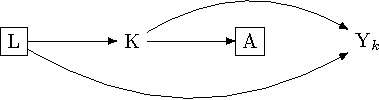
\includegraphics[width=1\textwidth,height=\textheight]{causal-dags_files/figure-pdf/fig_dag_multiple_version_treatment_dag-1.pdf}

}

\caption{Multiple Versions of treatment. Heae, A is regarded to bbe a
coarseneed version of K}

\end{figure}

Perhaps not all is lost. VanderWeele looks to the theory of multiple
versions of treatment for solace.

Recall, a causal effect is defined as the difference in the expected
potential outcome when everyone is exposed (perhaps contrary to fact) to
one level of a treatment, conditional on their levels of a confounder,
with the expected potential outcome when everyone is exposed to a a
different level of a treatement (perhaps contrary to fact), conditional
on their levels of a counfounder.

\[ \delta = \sum_l \left( \mathbb{E}[Y|A=a,l] - \mathbb{E}[Y|A=a^*,l] \right) P(l)\]

where \(\delta\) is the causal estimand on the difference scale
\((\mathbb{E}[Y^0 - Y^0])\).

In causal inference, the multiple versions of treatment theory allows us
to handle situations where the treatment isn not uniform, but instead
has several variations. Each variation or ``version'' of the treatment
can have a different effect on the outcome. However, consistency is not
violated because it is redefined: for each version of the treatment, the
outcome under that version is equal to the observed outcome when that
version is received. Put differently we may think of the indicator \(A\)
as corresponding to many version of the true treament \(K\). Where
conditional independence holds such that there is a absence of
confounding for the effect of \(K\) on \(Y\) given \(L\), we have:
\(Y(k)\coprod A|K,L\). This states conditional on \(L\), \(A\) gives no
information about \(Y\) once \(K\) and \(L\) are accounted for. When
\(Y = Y(k)\) if \(K = k\) and Y\((k)\) is independent of \(K\),
condition on \(L\), then \(A\) may be thought of as a coarsened
indicator of \(K\), as shown in
(\protect\hyperlink{ref-fig_dag_multiple_version_treatment_dag}{\textbf{fig\_dag\_multiple\_version\_treatment\_dag?}})
We may estimate consistent causal effects where:

\[ \delta = \sum_{k,l} \mathbb{E}[Y(k)|l] P(k|a,l) P(l) - \sum_{k,l} \mathbb{E}[Y(k)|l] P(k|a^*,l) P(l)\]

The scenario represents a hypothetical randomised trial where within
strata of covariates \(L\), individuals in one group receive a treatment
\(K\) version randomly assigned from the distribution of \(K\)
distribution \((A = 1, L = l)\) sub-population. Meanwhile, individuals
in the other group receive a randomly assigned \(K\) version from
\((A = 0, L = l)\)

This theory finds its utility in scenarios where treatments seldom
resemble each other (see: (\protect\hyperlink{ref-vanderweele2013}{Tyler
J. VanderWeele and Hernan 2013})).

\hypertarget{references}{%
\section*{References}\label{references}}
\addcontentsline{toc}{section}{References}

\hypertarget{refs}{}
\begin{CSLReferences}{1}{0}
\leavevmode\vadjust pre{\hypertarget{ref-bareinboim2022a}{}}%
Bareinboim, Elias, Jin Tian, and Judea Pearl. 2022. {``Recovering from
Selection Bias in Causal and Statistical Inference.''} In, 1st ed.,
36:433450. New York, NY, USA: Association for Computing Machinery.
\url{https://doi.org/10.1145/3501714.3501740}.

\leavevmode\vadjust pre{\hypertarget{ref-barrett2021}{}}%
Barrett, Malcolm. 2021. \emph{Ggdag: Analyze and Create Elegant Directed
Acyclic Graphs}. \url{https://CRAN.R-project.org/package=ggdag}.

\leavevmode\vadjust pre{\hypertarget{ref-basten2013}{}}%
Basten, Christoph, and Frank Betz. 2013. {``Beyond Work Ethic: Religion,
Individual, and Political Preferences.''} \emph{American Economic
Journal: Economic Policy} 5 (3): 67--91.
\url{https://doi.org/10.1257/pol.5.3.67}.

\leavevmode\vadjust pre{\hypertarget{ref-becker2016}{}}%
Becker, Sascha O, Steven Pfaff, and Jared Rubin. 2016. {``Causes and
Consequences of the Protestant Reformation.''} \emph{Explorations in
Economic History} 62: 125.

\leavevmode\vadjust pre{\hypertarget{ref-breskin2021}{}}%
Breskin, Alexander, Andrew Edmonds, Stephen R. Cole, Daniel Westreich,
Jennifer Cocohoba, Mardge H. Cohen, Seble G. Kassaye, et al. 2021.
{``G-computation for policy-relevant effects of interventions on
time-to-event outcomes.''} \emph{International Journal of Epidemiology}
49 (6): 2021--29. \url{https://doi.org/10.1093/ije/dyaa156}.

\leavevmode\vadjust pre{\hypertarget{ref-bulbulia2022}{}}%
Bulbulia, Joseph A. 2022. {``A Workflow for Causal Inference in
Cross-Cultural Psychology.''} \emph{Religion, Brain \& Behavior} 0 (0):
1--16. \url{https://doi.org/10.1080/2153599X.2022.2070245}.

\leavevmode\vadjust pre{\hypertarget{ref-chatton2020}{}}%
Chatton, Arthur, Florent Le Borgne, Clémence Leyrat, Florence
Gillaizeau, Chloé Rousseau, Laetitia Barbin, David Laplaud, Maxime
Léger, Bruno Giraudeau, and Yohann Foucher. 2020. {``G-Computation,
Propensity Score-Based Methods, and Targeted Maximum Likelihood
Estimator for Causal Inference with Different Covariates Sets: A
Comparative Simulation Study.''} \emph{Scientific Reports} 10 (1): 9219.
\url{https://doi.org/10.1038/s41598-020-65917-x}.

\leavevmode\vadjust pre{\hypertarget{ref-cinelli2022}{}}%
Cinelli, Carlos, Andrew Forney, and Judea Pearl. 2022. {``A Crash Course
in Good and Bad Controls.''} \emph{Sociological Methods \& Research},
May, 00491241221099552. \url{https://doi.org/10.1177/00491241221099552}.

\leavevmode\vadjust pre{\hypertarget{ref-cole2010}{}}%
Cole, Stephen R, Robert W Platt, Enrique F Schisterman, Haitao Chu,
Daniel Westreich, David Richardson, and Charles Poole. 2010.
{``Illustrating Bias Due to Conditioning on a Collider.''}
\emph{International Journal of Epidemiology} 39 (2): 417--20.
\url{https://doi.org/10.1093/ije/dyp334}.

\leavevmode\vadjust pre{\hypertarget{ref-danaei2012}{}}%
Danaei, Goodarz, Mohammad Tavakkoli, and Miguel A. Hernán. 2012. {``Bias
in observational studies of prevalent users: lessons for comparative
effectiveness research from a meta-analysis of statins.''}
\emph{American Journal of Epidemiology} 175 (4): 250--62.
\url{https://doi.org/10.1093/aje/kwr301}.

\leavevmode\vadjust pre{\hypertarget{ref-decoulanges1903}{}}%
De Coulanges, Fustel. 1903. \emph{La Cité Antique: Étude Sur Le Culte,
Le Droit, Les Institutions de La Grèce Et de Rome}. Hachette.

\leavevmode\vadjust pre{\hypertarget{ref-deffner2022a}{}}%
Deffner, Dominik, Julia M. Rohrer, and Richard McElreath. 2022. {``A
Causal Framework for Cross-Cultural Generalizability.''} \emph{Advances
in Methods and Practices in Psychological Science} 5 (3):
25152459221106366. \url{https://doi.org/10.1177/25152459221106366}.

\leavevmode\vadjust pre{\hypertarget{ref-duxedaz2021}{}}%
Díaz, Iván, Nicholas Williams, Katherine L. Hoffman, and Edward J.
Schenck. 2021. {``Non-Parametric Causal Effects Based on Longitudinal
Modified Treatment Policies.''} \emph{Journal of the American
Statistical Association}.
\url{https://doi.org/10.1080/01621459.2021.1955691}.

\leavevmode\vadjust pre{\hypertarget{ref-edwards2015}{}}%
Edwards, Jessie K, Stephen R Cole, and Daniel Westreich. 2015. {``All
Your Data Are Always Missing: Incorporating Bias Due to Measurement
Error into the Potential Outcomes Framework.''} \emph{International
Journal of Epidemiology} 44 (4): 14521459.

\leavevmode\vadjust pre{\hypertarget{ref-greenlands.1977a}{}}%
Greenland, S. 1977. {``Response and Follow-up Bias in Cohort Studies.''}
\emph{American Journal of Epidemiology} 106 (3): 184--87.
\url{https://doi.org/10.1093/oxfordjournals.aje.a112451}.

\leavevmode\vadjust pre{\hypertarget{ref-greenland1999}{}}%
Greenland, S., J. Pearl, and J. M. Robins. 1999. {``Causal diagrams for
epidemiologic research.''} \emph{Epidemiology (Cambridge, Mass.)} 10
(1): 37--48.

\leavevmode\vadjust pre{\hypertarget{ref-hernan2023}{}}%
Hernan, M. A., and J. M. Robins. 2023a. \emph{Causal Inference}. Chapman
\& Hall/CRC Monographs on Statistics \& Applied Probab. Taylor \&
Francis. \url{https://books.google.co.nz/books?id=/_KnHIAAACAAJ}.

\leavevmode\vadjust pre{\hypertarget{ref-hernan2023b}{}}%
---------. 2023b. \emph{Causal Inference}. Chapman \& Hall/CRC
Monographs on Statistics \& Applied Probab. Taylor \& Francis.
\url{https://books.google.co.nz/books?id=/_KnHIAAACAAJ}.

\leavevmode\vadjust pre{\hypertarget{ref-hernuxe1n2004}{}}%
Hernán, M. A. 2004. {``A Definition of Causal Effect for Epidemiological
Research.''} \emph{Journal of Epidemiology \& Community Health} 58 (4):
265--71. \url{https://doi.org/10.1136/jech.2002.006361}.

\leavevmode\vadjust pre{\hypertarget{ref-hernuxe1n2017}{}}%
---------. 2017. {``Invited Commentary: Selection Bias Without Colliders
\textbar{} American Journal of Epidemiology \textbar{} Oxford
Academic.''} \emph{American Journal of Epidemiology} 185 (11): 10481050.
\url{https://doi.org/10.1093/aje/kwx077}.

\leavevmode\vadjust pre{\hypertarget{ref-hernuxe1n2008a}{}}%
Hernán, Miguel A., Alvaro Alonso, Roger Logan, Francine Grodstein, Karin
B. Michels, Walter C. Willett, JoAnn E. Manson, and James M. Robins.
2008. {``Observational Studies Analyzed Like Randomized Experiments: An
Application to Postmenopausal Hormone Therapy and Coronary Heart
Disease.''} \emph{Epidemiology} 19 (6): 766.
\url{https://doi.org/10.1097/EDE.0b013e3181875e61}.

\leavevmode\vadjust pre{\hypertarget{ref-hernuxe1n2009}{}}%
Hernán, Miguel A., and Stephen R. Cole. 2009. {``Invited Commentary:
Causal Diagrams and Measurement Bias.''} \emph{American Journal of
Epidemiology} 170 (8): 959--62.
\url{https://doi.org/10.1093/aje/kwp293}.

\leavevmode\vadjust pre{\hypertarget{ref-hernuxe1n2004b}{}}%
Hernán, Miguel A., Sonia Hernández-Díaz, and James M. Robins. 2004. {``A
Structural Approach to Selection Bias.''} \emph{Epidemiology} 15 (5):
615--25. \url{https://www.jstor.org/stable/20485961}.

\leavevmode\vadjust pre{\hypertarget{ref-hernuxe1n2006}{}}%
Hernán, Miguel A., and James M. Robins. 2006. {``Estimating Causal
Effects from Epidemiological Data.''} \emph{Journal of Epidemiology \&
Community Health} 60 (7): 578--86.
\url{https://doi.org/10.1136/jech.2004.029496}.

\leavevmode\vadjust pre{\hypertarget{ref-hernuxe1n2016a}{}}%
Hernán, Miguel A, Brian C Sauer, Sonia Hernández-Díaz, Robert Platt, and
Ian Shrier. 2016. {``Specifying a Target Trial Prevents Immortal Time
Bias and Other Self-Inflicted Injuries in Observational Analyses.''}
\emph{Journal of Clinical Epidemiology} 79: 7075.

\leavevmode\vadjust pre{\hypertarget{ref-hernuxe1n2022a}{}}%
Hernán, Miguel A., Wei Wang, and David E. Leaf. 2022. {``Target Trial
Emulation: A Framework for Causal Inference from Observational Data.''}
\emph{JAMA} 328 (24): 2446--47.
\url{https://doi.org/10.1001/jama.2022.21383}.

\leavevmode\vadjust pre{\hypertarget{ref-holland1986}{}}%
Holland, Paul W. 1986. {``Statistics and Causal Inference.''}
\emph{Journal of the American Statistical Association} 81 (396): 945960.

\leavevmode\vadjust pre{\hypertarget{ref-lu2022a}{}}%
Lu, Haidong, Stephen R. Cole, Chanelle J. Howe, and Daniel Westreich.
2022. {``Toward a Clearer Definition of Selection Bias When Estimating
Causal Effects.''} \emph{Epidemiology (Cambridge, Mass.)} 33 (5):
699--706. \url{https://doi.org/10.1097/EDE.0000000000001516}.

\leavevmode\vadjust pre{\hypertarget{ref-mcelreath2020}{}}%
McElreath, Richard. 2020. \emph{Statistical Rethinking: A Bayesian
Course with Examples in r and Stan}. CRC press.

\leavevmode\vadjust pre{\hypertarget{ref-naimi2017}{}}%
Naimi, Ashley I, Stephen R Cole, and Edward H Kennedy. 2017. {``An
Introduction to g Methods.''} \emph{International Journal of
Epidemiology} 46 (2): 756--62. \url{https://doi.org/10.1093/ije/dyw323}.

\leavevmode\vadjust pre{\hypertarget{ref-pearl2009}{}}%
Pearl, Judea. 2009. {``Causal Inference in Statistics: An Overview.''}
\url{https://doi.org/10.1214/09-SS057}.

\leavevmode\vadjust pre{\hypertarget{ref-richardson2013}{}}%
Richardson, Thomas S, and James M Robins. 2013. {``Single World
Intervention Graphs: A Primer.''} In. Citeseer.

\leavevmode\vadjust pre{\hypertarget{ref-robins}{}}%
Robins, James M, and Miguel A Hernán. n.d. {``Estimation of the Causal
Effects of Time-Varying Exposures.''}

\leavevmode\vadjust pre{\hypertarget{ref-rohrer2018}{}}%
Rohrer, Julia M. 2018. {``Thinking Clearly about Correlations and
Causation: Graphical Causal Models for Observational Data.''}
\emph{Advances in Methods and Practices in Psychological Science} 1 (1):
2742.

\leavevmode\vadjust pre{\hypertarget{ref-rubin1976}{}}%
Rubin, D. B. 1976. {``Inference and Missing Data.''} \emph{Biometrika}
63 (3): 581--92. \url{https://doi.org/10.1093/biomet/63.3.581}.

\leavevmode\vadjust pre{\hypertarget{ref-shi2021}{}}%
Shi, Baoyi, Christine Choirat, Brent A Coull, Tyler J VanderWeele, and
Linda Valeri. 2021. {``CMAverse: A Suite of Functions for Reproducible
Causal Mediation Analyses.''} \emph{Epidemiology} 32 (5): e20e22.

\leavevmode\vadjust pre{\hypertarget{ref-suzuki2016}{}}%
Suzuki, Etsuji, Toshiharu Mitsuhashi, Toshihide Tsuda, and Eiji
Yamamoto. 2016. {``A Typology of Four Notions of Confounding in
Epidemiology.''} \emph{Journal of Epidemiology} 27 (2): 49--55.
\url{https://doi.org/10.1016/j.je.2016.09.003}.

\leavevmode\vadjust pre{\hypertarget{ref-suzuki2020}{}}%
Suzuki, Etsuji, Tomohiro Shinozaki, and Eiji Yamamoto. 2020. {``Causal
Diagrams: Pitfalls and Tips.''} \emph{Journal of Epidemiology} 30 (4):
153--62. \url{https://doi.org/10.2188/jea.JE20190192}.

\leavevmode\vadjust pre{\hypertarget{ref-suzuki2014}{}}%
Suzuki, Etsuji, and Eiji Yamamoto. 2014. {``Further Refinements to the
Organizational Schema for Causal Effects.''} \emph{Epidemiology} 25 (4):
618. \url{https://doi.org/10.1097/EDE.0000000000000114}.

\leavevmode\vadjust pre{\hypertarget{ref-swanson1967}{}}%
Swanson, Guy E. 1967. {``Religion and Regime: A Sociological Account of
the Reformation.''}

\leavevmode\vadjust pre{\hypertarget{ref-swanson1971}{}}%
Swanson, Guy E. 1971. {``Interpreting the Reformation.''} \emph{The
Journal of Interdisciplinary History} 1 (3): 419446.
\url{http://www.jstor.org/stable/202620}.

\leavevmode\vadjust pre{\hypertarget{ref-tripepi2007}{}}%
Tripepi, G., K. J. Jager, F. W. Dekker, C. Wanner, and C. Zoccali. 2007.
{``Measures of Effect: Relative Risks, Odds Ratios, Risk Difference, and
{`}Number Needed to Treat{'}.''} \emph{Kidney International} 72 (7):
789--91. \url{https://doi.org/10.1038/sj.ki.5002432}.

\leavevmode\vadjust pre{\hypertarget{ref-vanderweele2015}{}}%
VanderWeele, Tyler. 2015a. \emph{Explanation in Causal Inference:
Methods for Mediation and Interaction}. Oxford University Press.

\leavevmode\vadjust pre{\hypertarget{ref-vanderweele2015a}{}}%
---------. 2015b. \emph{Explanation in Causal Inference: Methods for
Mediation and Interaction}. Oxford University Press.

\leavevmode\vadjust pre{\hypertarget{ref-vanderweele2019a}{}}%
VanderWeele, Tyler J. 2019. {``Principles of Confounder Selection.''}
\emph{European Journal of Epidemiology} 34 (3): 211219.

\leavevmode\vadjust pre{\hypertarget{ref-vanderweele2009}{}}%
VanderWeele, Tyler J. 2009. {``Concerning the Consistency Assumption in
Causal Inference.''} \emph{Epidemiology} 20 (6): 880.
\url{https://doi.org/10.1097/EDE.0b013e3181bd5638}.

\leavevmode\vadjust pre{\hypertarget{ref-vanderweele2012}{}}%
---------. 2012. {``Confounding and Effect Modification: Distribution
and Measure.''} \emph{Epidemiologic Methods} 1 (1): 55--82.
\url{https://doi.org/10.1515/2161-962X.1004}.

\leavevmode\vadjust pre{\hypertarget{ref-vanderweele2018}{}}%
---------. 2018. {``On Well-Defined Hypothetical Interventions in the
Potential Outcomes Framework.''} \emph{Epidemiology} 29 (4): e24.
\url{https://doi.org/10.1097/EDE.0000000000000823}.

\leavevmode\vadjust pre{\hypertarget{ref-vanderweele2022}{}}%
---------. 2022a. {``Constructed Measures and Causal Inference: Towards
a New Model of Measurement for Psychosocial Constructs.''}
\emph{Epidemiology} 33 (1): 141.
\url{https://doi.org/10.1097/EDE.0000000000001434}.

\leavevmode\vadjust pre{\hypertarget{ref-vanderweele2022a}{}}%
---------. 2022b. {``Constructed Measures and Causal Inference: Towards
a New Model of Measurement for Psychosocial Constructs.''}
\emph{Epidemiology} 33 (1): 141.
\url{https://doi.org/10.1097/EDE.0000000000001434}.

\leavevmode\vadjust pre{\hypertarget{ref-vanderweele2013}{}}%
VanderWeele, Tyler J, and Miguel A Hernan. 2013. {``Causal Inference
Under Multiple Versions of Treatment.''} \emph{Journal of Causal
Inference} 1 (1): 120.

\leavevmode\vadjust pre{\hypertarget{ref-vanderweele2012a}{}}%
VanderWeele, Tyler J., and Miguel A. Hernán. 2012. {``Results on
Differential and Dependent Measurement Error of the Exposure and the
Outcome Using Signed Directed Acyclic Graphs.''} \emph{American Journal
of Epidemiology} 175 (12): 1303--10.
\url{https://doi.org/10.1093/aje/kwr458}.

\leavevmode\vadjust pre{\hypertarget{ref-vanderweele2014}{}}%
VanderWeele, Tyler J, and Mirjam J Knol. 2014. {``A Tutorial on
Interaction.''} \emph{Epidemiologic Methods} 3 (1): 3372.

\leavevmode\vadjust pre{\hypertarget{ref-vanderweele2020}{}}%
VanderWeele, Tyler J, Maya B Mathur, and Ying Chen. 2020.
{``Outcome-Wide Longitudinal Designs for Causal Inference: A New
Template for Empirical Studies.''} \emph{Statistical Science} 35 (3):
437466.

\leavevmode\vadjust pre{\hypertarget{ref-vanderweele2007}{}}%
VanderWeele, Tyler J., and James M. Robins. 2007. {``Four types of
effect modification: a classification based on directed acyclic
graphs.''} \emph{Epidemiology (Cambridge, Mass.)} 18 (5): 561--68.
\url{https://doi.org/10.1097/EDE.0b013e318127181b}.

\leavevmode\vadjust pre{\hypertarget{ref-vanderweele2022b}{}}%
VanderWeele, Tyler J, and Stijn Vansteelandt. 2022. {``A Statistical
Test to Reject the Structural Interpretation of a Latent Factor
Model.''} \emph{Journal of the Royal Statistical Society Series B:
Statistical Methodology} 84 (5): 20322054.

\leavevmode\vadjust pre{\hypertarget{ref-watts2016}{}}%
Watts, J., O. Sheehan, Q. D. Atkinson, J., and R. D. Gray. 2016.
{``Ritual Human Sacrifice Promoted and Sustained the Evolution of
Stratified Societies.''} \emph{Nature} 532 (7598): 228231.

\leavevmode\vadjust pre{\hypertarget{ref-weber1905}{}}%
Weber, Max. 1905. \emph{The Protestant Ethic and the Spirit of
Capitalism: And Other Writings}. Penguin.

\leavevmode\vadjust pre{\hypertarget{ref-weber1993}{}}%
---------. 1993. \emph{The Sociology of Religion}. Beacon Press.

\leavevmode\vadjust pre{\hypertarget{ref-westreich2010}{}}%
Westreich, Daniel, and Stephen R. Cole. 2010. {``Invited commentary:
positivity in practice.''} \emph{American Journal of Epidemiology} 171
(6). \url{https://doi.org/10.1093/aje/kwp436}.

\leavevmode\vadjust pre{\hypertarget{ref-westreich2015}{}}%
Westreich, Daniel, Jessie K Edwards, Stephen R Cole, Robert W Platt,
Sunni L Mumford, and Enrique F Schisterman. 2015. {``Imputation
Approaches for Potential Outcomes in Causal Inference.''}
\emph{International Journal of Epidemiology} 44 (5): 17311737.

\leavevmode\vadjust pre{\hypertarget{ref-wheatley1971}{}}%
Wheatley, Paul. 1971. \emph{The Pivot of the Four Quarters : A
Preliminary Enquiry into the Origins and Character of the Ancient
Chinese City}. Edinburgh University Press.
\url{https://cir.nii.ac.jp/crid/1130000795717727104}.

\leavevmode\vadjust pre{\hypertarget{ref-williams2021}{}}%
Williams, Nicholas T., and Iván Díaz. 2021. \emph{Lmtp: Non-Parametric
Causal Effects of Feasible Interventions Based on Modified Treatment
Policies}. \url{https://doi.org/10.5281/zenodo.3874931}.

\end{CSLReferences}



\end{document}
